\documentclass{article}
\usepackage[left=0.85in, right=0.85in, top=0.5in, bottom=0.95in]{geometry}
\usepackage[T1]{fontenc}
\usepackage[utf8]{inputenc}
\usepackage[italian]{babel}
\usepackage{graphicx}
\usepackage{wrapfig2}
\usepackage{amsmath}
\usepackage{amsthm} %teoremi
\usepackage{cancel}
\usepackage{amssymb}
\usepackage{cases}
\usepackage{subcaption}
\usepackage{hyperref}
\hypersetup{
	colorlinks=true,
	linkcolor=blue,    
	urlcolor=blue,
	pdfpagemode=FullScreen,
}
\urlstyle{same}
\usepackage{changepage}
\usepackage{lastpage, epstopdf}
\usepackage{fancyhdr}
\usepackage{tcolorbox}
\usepackage{background}


%=======HEADER & FOOTER=======%
\def\lesson{Lesson Title}
%\def\outcome{\textbf{Learning Outcomes:} Outcomes go here. }

%\pagestyle{fancy}
%\fancyhf{}
%\renewcommand{\headrulewidth}{0pt}
%\renewcommand{\footrulewidth}{1.4pt}
%\lfoot{My Name $\diamond$ \the\year}
%\cfoot{Page \thepage/\pageref{LastPage}}
%\rfoot{\lesson}

%=======CORNELL STYLE FORMAT=======%
\SetBgScale{1}
\SetBgAngle{0}
\SetBgColor{black}
\SetBgContents{\rule{1pt}{0.899\paperheight}}
\SetBgHshift{-1.6in}
\SetBgVshift{-0.1in}

%=======CUSTOM BOXES=======%

\parindent 0ex

%=======BODY=======%

%=======TEOREMI=======%
\newtheorem*{thm}{Teorema} 
\newtheorem*{oss}{Osservazione}
\newtheorem*{definition}{Definizione}

\begin{document}
	%	\setcounterpageref{secnumdepth}{0}
	\section*{MECCANICA DEI SOLIDI: PARTE 7} %Date: \hrulefill}
%	\begin{tcolorbox}{\outcome}\end{tcolorbox}


\begin{adjustwidth}{2in}{} 
{\Large \textbf{Meccanica del continuo}} \mbox{} \newline
\textbf{Analisi dello stato di tensione} \newline

	Dal globale al locale: come si traduce una determinata caratteristica della sollecitazione? in che stato tensionale? Come viene sollecitato il materiale al suo interno? \newline 
	
	Si rimuove l'ipotesi per cui si aveva a che fare con corpi dal comportamento rigido, in questo modo l'analisi dello stato di tensione diviene l'analisi degli effetti interni del materiale che essendo questo deformabile, viene soggetto a carichi esterni tradotti in caratteristiche della sollecitazione. \newline
	
	La seguente trattazione è effettuata sotto le ipotesi di piccoli spostamenti, ovvero di spostamenti dovuti alle deformazioni del corpo (CHE NON SONO MOTI RIGIDI) piccoli rispetto alle dimensioni dell'oggetto. 
	
	In questo modo si può analizzare sia nella configurazione iniziale che in quella finale una geometria pari a quella indeformata, ovvero la forma iniziale. \newline 
	
	Si consideri il caso generico di un solido tridimensionale soggetto a due risultanti:

	\begin{itemize}
		\item  delle forze di volume $f(x,y,z)$
		\item  delle forze di superficie $p(x,y,z)$
	\end{itemize}

	Si analizzi il solido  nella sua configurazione indeformata, considerando cioè 
	trascurabili gli spostamenti dei punti del solido dovuti all’applicazione dei carchi.
	
	Si consideri un solido deformabile \underline{in equilibrio} sotto l’azione di forze esterne:
	
\begin{figure}[H]
	\centering
	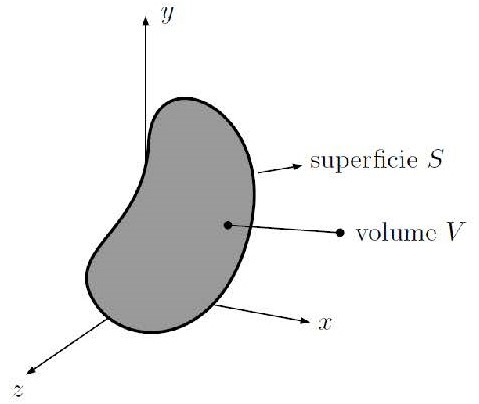
\includegraphics[width=0.3\linewidth]{immagini/1.PARTE7_Pagina_02}
\end{figure}

	\[ \int_{S}p(x,y,z)dS + \int_{V}f(x,y,z)dV = 0  \]

	Si tagli il solido considerato con un piano A. \newline 
	
	Sulla faccia di sezione nascerebbero delle caratteristiche della sollecitazione che equilibrerebbero le azioni esterne sulla porzione considerata. 
	
	Queste caratteristiche della sollecitazione si possono vedere come una distribuzione di vettori $t$, forze di superficie, che si instaurano sulla superficie di separazione con una certa distribuzione, con una legge variabile in $x,y,z$. \newline 
	
	Se il solido di partenza era in equilibrio, ciascuno dei due solidi così ottenuti rimarrà in equilibrio.\newline
	
	Si suppone così la presenza sul piano di
	sezione di forze superficiali $ t(x,y,z) $.

\begin{figure}[H]
	\centering
	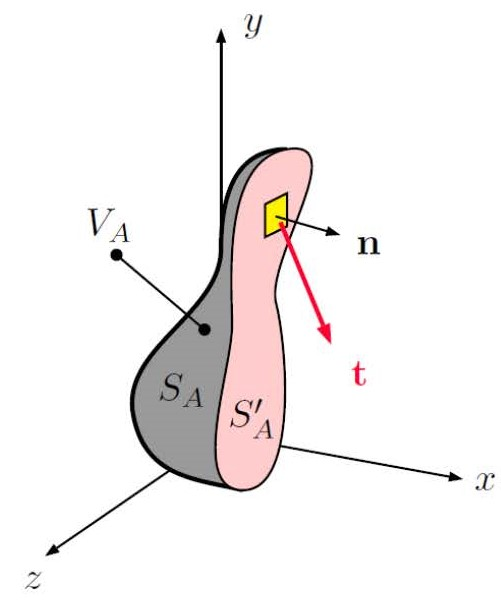
\includegraphics[width=0.3\linewidth]{immagini/1.PARTE7_Pagina_03}
\end{figure}
	Eseguito il taglio c'è una nuova superficie sulla quale nascono delle tensioni $t$ la cui risultante è una forza che equilibra le forze esterne, superficiali e volumetriche. \newline
	
	Indicando con $ S_A $ la superficie esterna di uno dei due
	solidi, con $ S'_A $ la superficie della sezione e con $ V_A $ il
	relativo volume, si ha:
	
	\[ \int_{S_A}p(x,y,z)dS + \int_{S'_A}t(x,y,z)dS + \int_{V}f(x,y,z)dV = 0  \]
		
	Se si individuasse un punto P della sezione, individuato  questo dal vettore
	posizione $\vec{r}(x,y,z)$, il punto P sarà caratterizzato da un suo vettore $t$ che ne indicherà lo stato tensionale: $t$ caratterizza lo stato tensionale in P rispetto alla giacitura di normale $\hat{n}$, quel vettore è perciò valido quando per P passa quel piano di sezione. Allora le forze di
	superficie $ t $ dipenderà anche dalla giacitura
	del piano di sezione:
	
	\[ t(\vec{r}, \hat{n})\]
	
	Poiché per un punto passano infiniti piani si hanno infinite giaciture $\vec{n}$ e quindi infiniti valori di $ t_n $: il suo complesso costituisce proprio lo stato di tensione in P. \newline
	
	Si individuano allora 3 piani, quello di normale $x$, quello di normale $y$ e quello di normale $z$. 
	
	Si supponga di conoscere i valori di $ t $ nel punto P lungo le tre giaciture
	dalle basi del sistema di riferimento ortonormale individuato, si trova, come primo componente riportato $t_x$, il vettore tensione nel punto P quando per P passa un piano di normale/giacitura $x$, e cosi per $t_y$ e $t_z$:
	
	\[
	t_x = \left( \begin{array}{c}
		t_{xx} \\
		t_{xy} \\
		t_{xz}
	\end{array}\right)  \hspace{1cm} 	t_y =\left(  \begin{array}{c}
		t_{yx} \\
		t_{yy} \\
		t_{yz}
	\end{array}\right)  \hspace{1cm} t_z = \left( \begin{array}{c}
		t_{zx} \\
		t_{zy} \\
		t_{zz}
	\end{array}\right) 
	\]
	
	In cui si possono ulteriormente individuare i tre valori di $ t $ nel punto P lungo le giaciture perpendicolari, rispettivamente, alle basi
	$\hat{i}$, $\hat{j}$ e $\hat{k}$.
	
\begin{figure}[H]
	\centering
	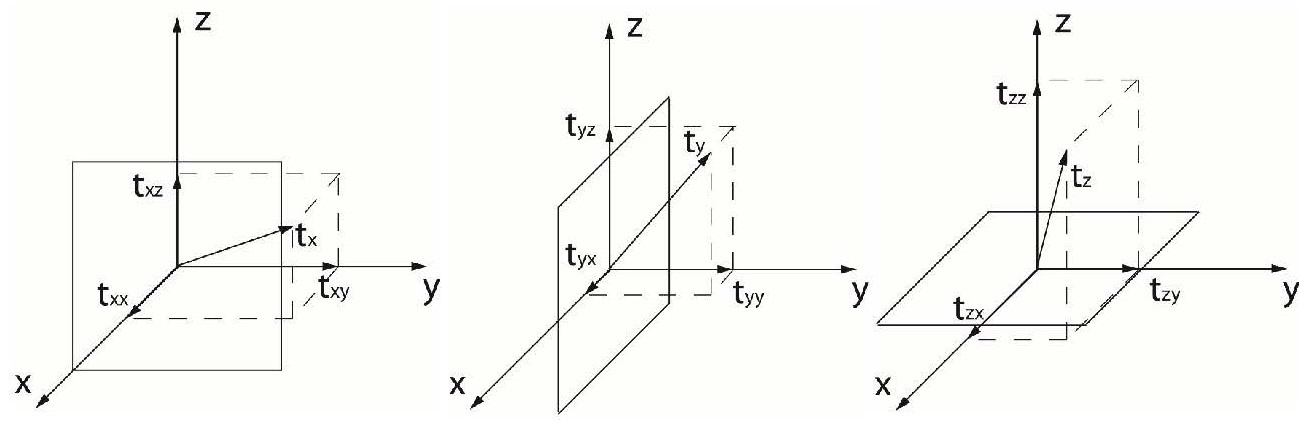
\includegraphics[width=0.6\linewidth]{immagini/1.PARTE7_Pagina_04}
\end{figure}
	Si prenda ad esempio il vettore $t_z$, quel vettore di normale $\hat{z}$ può avere qualunque inclinazione, ma nel piano cartesiano centrato in P avrà componente $x, y, z$. \newline 
	
	
	Si noti come:
	\begin{itemize}
		\item Il primo indice caratterizza la giacitura;
		\item Il secondo indice descrive l'asse secondo il quale è diretta la componente;
		\item Le componendi di indici uguali sono le tensioni normali sulle tre giaciture;
		\item Le componenti con indice diverso cono invece le componenti di tensione tangenziale, giacciono nel piano della giacitura.
	\end{itemize}
\vspace{1cm}

{\Large \textbf{Teorema di Cauchy}}\newline
	Queste 9 componenti individuate - qualora siano note -  sono tutte quelle necessarie e sufficienti a descrivere lo stato di tensione in un punto P. \newline

	\begin{thm}
		La conoscenza delle tensioni su tre distinte giaciture in P è sufficiente a determinare la tensione su ogni altra giacitura in P. \newline
	\end{thm}	

	Se si assume come terna di giaciture quelle ortogonali all’asse, le tensioni che si
	suppongono note allora sono:
	
	\[
	t_x = \left( \begin{array}{c}
		t_{xx} \\
		t_{xy} \\
		t_{xz}
	\end{array}\right)  \hspace{1cm} 	t_y =\left(  \begin{array}{c}
		t_{yx} \\
		t_{yy} \\
		t_{yz}
	\end{array}\right)  \hspace{1cm} t_z = \left( \begin{array}{c}
		t_{zx} \\
		t_{zy} \\
		t_{zz}
	\end{array}\right) 
	\]
	
	Data una generica giacitura di normale $\hat{n}$, la tensione su di essa sarà:
	
		\[
	t_n = \left( \begin{array}{c}
		t_{nx} \\
		t_{ny} \\
		t_{nz}
	\end{array}\right) 
	\]

	 Per il Teorema di Cauchy, (gli $\hat{n}_i$ prendono anche il nome di coseni direttori): 
	 
	 \[
	 \begin{cases}
		t_{nx} = t_{xx}n_x + t_{yx}n_y + t_{zx}n_z \\
		t_{ny} = t_{xy}n_x + t_{yy}n_y + t_{zy}n_z \\
		t_{nz} = t_{xz}n_x + t_{yz}n_y + t_{zz}n_z \\
	 \end{cases}
	 \]
	 
	 Il teorema di Cauchy si può scrivere in forma compatta come una matrice 3x3:
	 
	 \[
	 	t_n = \left( \begin{array}{c}
	 	t_{nx} \\
	 	t_{ny} \\
	 	t_{nz}
	 \end{array}\right) = \left[ \begin{array}{ccc}
	 t_{xx} & t_{yx} & t_{zx} \\
	 t_{xy} & t_{yy} & t_{zy} \\
	 t_{xz} & t_{yz} & t_{zz}
 \end{array}\right] \left( \begin{array}{c}
 n_x \\
 n_y \\
 n_z
\end{array}\right) = [t] \hat{n}
	 \] 
	 
	 In cui $ [t] $ è il tensore degli sforzi, ben più noto nella seguente forma: 
	 
	 \[
	 [\sigma] = \left[ \begin{array}{ccc}
	 	\sigma_x & \tau_{yx} & \tau_{zx} \\
	 	\tau_{xy} & \sigma_y & \tau_{zy} \\
	 	\tau_{xz} & \tau_{yz} & \sigma_z
	 \end{array}\right]
	 \] 
	 Dove le $\tau$ sono le azioni tangenziali nel piano di giacitura e le $\sigma$ sono le azioni normali. \newpage
\begin{proof}(Teorema di Cauchy)
		 
	 Ci si ricava nel corpo di partenza un volume infinitesimo. 
	 
	 Si consideri perciò un tetraedro
	 infinitesimo con un vertice nel
	 punto P, tre facce normali agli
	 assi e una quarta secondo la
	 giacitura $\hat{n}$ obliqua, generica.
	 
\begin{figure}[H]
	\centering
	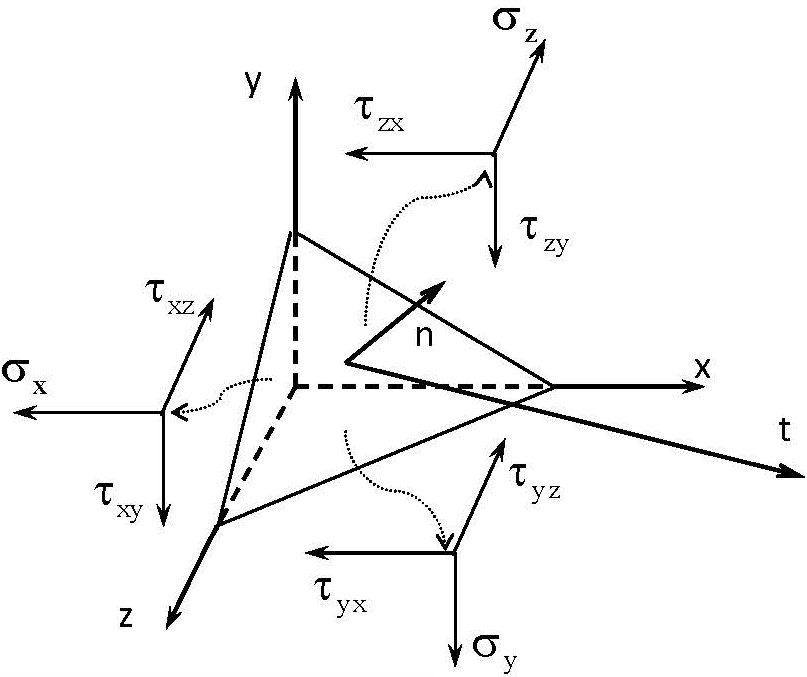
\includegraphics[width=0.4\linewidth]{immagini/1.PARTE7_Pagina_08 (2)}
\end{figure}
	Dato che il volume da cui è stato estratto il tetraedro è in equilibrio, sarà in equilibrio anche in tetraedro. 
	
	Si avrà allora uno stato tensionale tale che sulle facce di separazione si può leggere una distribuzione di tensione che mantenga in equilibrio il volume infinitesimo. \newline 
	
	 Nota $ dA $ l’area della giacitura in $\hat{n}$ le altre aree saranno: 
	 
	 \[
	 \begin{split}
		dA_x & = dA n_x \\
				dA_y & = dA n_y \\
						dA_z & = dA n_z \\
	 \end{split}
	 \]
	 
	 Si scriva - uno per tutti - l'equilibrio a traslazione in direzione $x$: 

\begin{figure}[H]
	\centering
	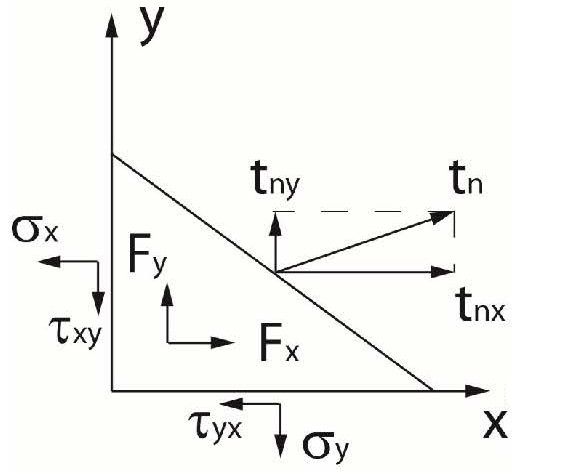
\includegraphics[width=0.4\linewidth]{immagini/1.PARTE7_Pagina_08}
\end{figure}	 
	 \[ 
	 t_{nx}dA - \sigma_x dA n_x - \tau_{yx} dA n_y - \tau_{zx} dA n_z + F_xdV = 0
	 \]
	 Ricordando che il tetraedro è infinitesimo: 
	 \[
	 dV \rightarrow 0
	 \]
	 Si giunge a: 
	 \[ 
	 t_{nx} = \sigma_x n_x +\tau_{yx} n_y + \tau_{zx} n_z 
	 \]
	 Equivalentemente per le altre direzioni.
\end{proof}
	 \newpage
\begin{proof} (\textbf{Simmetria dello stato di tensione}) 
	
	Si dimostri che i termini diagonali del tensore delle tensioni di Cauchy siano uguali fra loro. \newline 
	
	Si consideri un parallelepipedo infinitesimo con un vertice nel punto P individuato
	dal vettore posizione $\vec{r}$ ed avente spigoli di lunghezza $dx, dy, dz$.	
\begin{figure}[H]
	\centering
	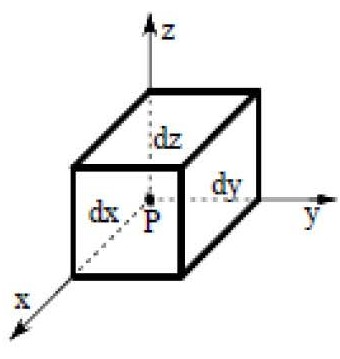
\includegraphics[width=0.2\linewidth]{immagini/1.PARTE7_Pagina_09 (2)}
\end{figure}
	Imponendo l'equilibrio a rotazione lungo un asse parallelo all'asse $ z $ e passante per il baricentro, si ottiene che il momento è esprimibile secondo:
	\[M = Fd = \tau A \cdot d\]
	Notare come i contributi $\sigma$ passino per l'asse di rotazione e quindi diano risultante a momento nulla.
	\begin{figure}[H]
		\centering
		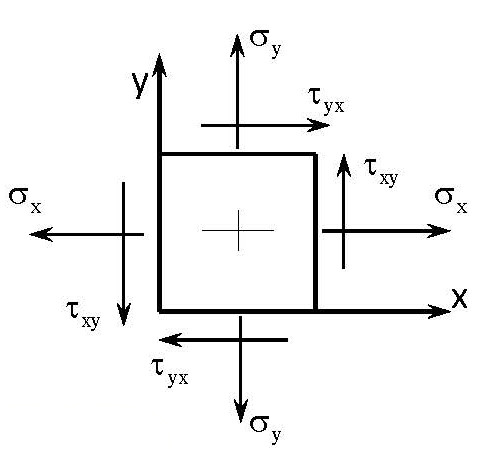
\includegraphics[width=0.3\linewidth]{immagini/1.PARTE7_Pagina_09}
	\end{figure}
	Allora l'equilibrio a momento diviene:
	\[
	\underbrace{\left(\tau_{xy}dzdy \right) dx }_{\text{oraria}}- \underbrace{\left(\tau_{yx}dxdz \right) dy}_{\text{antioraria}} = 0 \Rightarrow \tau_{xy} = \tau_{yx}
	\]
	
	Equivalentemente, per le altre componenti:
	
	\[
	\begin{split}
	\tau_{xz} & = \tau_{zx} \\
	\tau_{yz} & = \tau_{zy}
	\end{split}
	\]
	 E il tensore degli sforzi è simmetrico
\end{proof}	 
\newpage	 
{\Large \textbf{Equazioni indefinite di equilibrio alla traslazione}}\newline
	Un corpo globalmente in equilibrio è in equilibrio anche localmente: su di un corpo qualsiasi devono essere soddisfatte le equazioni di equilibrio locale. \newline 
	
	Le condizioni esterne agenti sul corpo in equilibrio devono soddisfare le equazioni
	cardinali della statica.
	
	 \[
	\begin{cases}
		\begin{aligned}
	\frac{\partial\sigma_x}{\partial x} + \frac{\partial \tau_{yx}}{\partial y} + \frac{\partial \tau_{zx}}{\partial z} + F_x & =0 \\
	
	\frac{\partial \tau_{xy}}{\partial x} + \frac{\partial\sigma_y}{\partial y} + \frac{\partial \tau_{zy}}{\partial z} + F_y & =0 \\
	
	\frac{\partial \tau_{xz}}{\partial x} + \frac{\partial \tau_{yz}}{\partial z} + \frac{\partial\sigma_z}{\partial z} + F_z & =0 \\
	\end{aligned}
	\end{cases}
	\]
	
	\[
	\nabla \cdot \sigma + \vec{F} = 0
	\]
	
	Sono dette equazioni indefinite di equilibrio alla traslazione. \newline 
	
	Se si è in grado di far rispettare queste equazioni di equilibrio in qualunque volume infinitesimo, allora il corpo deformabile è in equilibrio. 
	
	\begin{proof}
		
	
	Si consideri un parallelepipedo
	infinitesimo con un vertice in P e spigoli
	$ dx, dy, dz $, dato che è una porzione di corpo in equilibrio, allora dovrà essere in equilibrio, significa che sulle sue facce esterne nasceranno dei vettori tensione che garantiranno l'equilibrio. 
	
\begin{figure}[H]
	\centering
	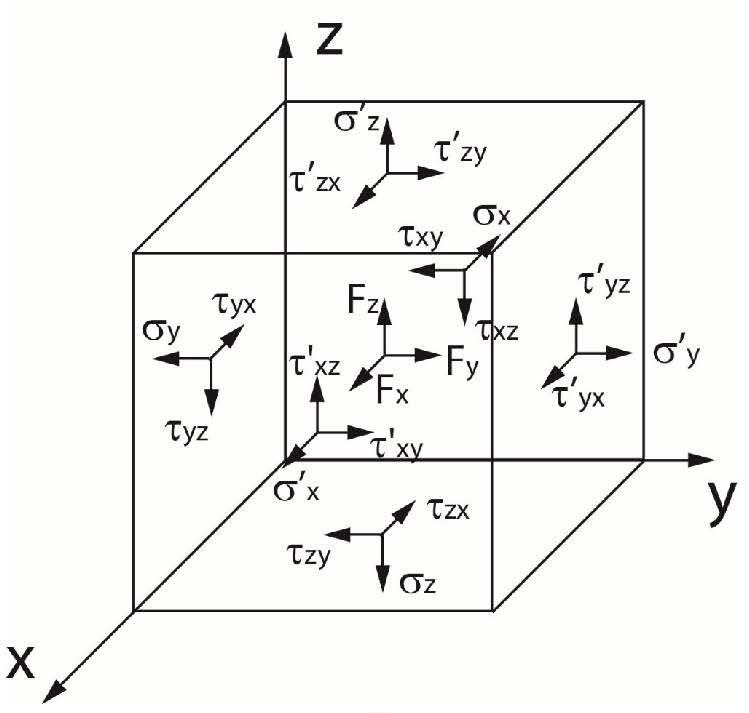
\includegraphics[width=0.3\linewidth]{immagini/1.PARTE7_Pagina_11}
\end{figure}
	\[
	\begin{array}{c}
		\begin{aligned}
		\sigma'_x & = \sigma_x + \frac{\partial \sigma_x}{\partial x} dx \\
		\tau'_{xy} & = \tau_{xy} + \frac{\partial \tau_{xy}}{\partial x} dx \\
		\tau'_{xz} & = \tau_{xz} + \frac{\partial \tau_{xz}}{\partial x} dx
		\end{aligned}
	\end{array} \hspace{1cm} \begin{array}{c}
	\begin{aligned}
		\sigma'_y & = \sigma_y + \frac{\partial \sigma_y}{\partial y} dy \\
		\tau'_{yx} & = \tau_{yx} + \frac{\partial \tau_{yx}}{\partial y} dy \\
		\tau'_{yz} & = \tau_{yz} + \frac{\partial \tau_{yz}}{\partial y} dy
	\end{aligned}
	\end{array} \hspace{1cm} \begin{array}{c}
	\begin{aligned}
		\sigma'_z & = \sigma_z + \frac{\partial \sigma_z}{\partial z} dz \\
		\tau'_{zx} & = \tau_{zx} + \frac{\partial \tau_{zx}}{\partial z} dz \\
		\tau'_{zy} & = \tau_{zy} + \frac{\partial \tau_{zy}}{\partial z} dz
	\end{aligned}
	\end{array}
	\]	
	
	Si imponga a questo punto l'equilibrio a traslazione in direzione x:
	
	\[
	\begin{split}
		-\sigma_x dydz & + \left( \sigma_x + \frac{\partial \sigma_x}{\partial x} dx\right) dydz - \tau_{yx}dxdz + \left( \tau_{yx} + \frac{\partial \tau_{yx}}{\partial y} dy\right) dxdz + \\
		-\tau_{zx} dxdy & + \left( \tau_{zx} + \frac{\partial \tau_{zx}}{\partial z} dz \right) dxdy + F_x dx dy dz = 0
	\end{split}
	\]
	Quello che rimane dopo le opportune semplificazione è: 
	
	\[
	\left( \frac{\partial \sigma_x}{\partial x} +  \frac{\partial \tau_{yx}}{\partial y} + \frac{\partial \tau_{zx}}{\partial z} + F_x \right) dxdydz = 0 
	\]
	
	E dunque: 
	
	\[
	\frac{\partial \sigma_x}{\partial x} +  \frac{\partial \tau_{yx}}{\partial y} + \frac{\partial \tau_{zx}}{\partial z} + F_x = 0	
	\]
	
	Analogamente per le altre direzioni.
	
	\end{proof}

	Queste equazioni valgono in ogni volume interno al corpo, ma se il volume interno al corpo è in equilibrio, lo sarà anche la superficie, c'è allora la necessità di trovare un equilibrio sul bordo del volume, tra le azioni esterne $\vec{p}$ e il tensore delle tensioni in quel punto. \newline
	
	Sono necessarie perciò ulteriori relazioni di
	equilibrio, valide in tutti i punti del contorno, che leghino le tensioni alle forze di
	superficie. \newline 
	
	Se il bordo è caratterizzato da $\hat{n}$ allora in quel punto dovrà essere valido il teorema di Cauchy. 

\begin{figure}[H]
	\centering
	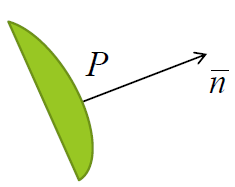
\includegraphics[width=0.15\linewidth]{immagini/Screenshot (86)}
\end{figure}
	Analogamente al Teorema di Cauchy considerando in questo caso le tensioni della generica giacitura come le forze di superficie applicate, si ottiene:
	 \[
	\begin{cases}
		p_x = \sigma_x n_x + \tau_{yx}n_y + \tau_{zx}n_z \\
		p_y = \tau_{xy}n_x + \sigma_y n_y + \tau_{zy}n_z \\
		p_z = \tau_{xz}n_x + \tau_{yz}n_y + \sigma_z n_z \\
	\end{cases}
	\]
	Ovvero il tenore pressione esterna $\vec{p}$ deve instaurare una condizione di equilibrio con le tensioni interne, queste espresse dei nove termini del tensore delle tensioni. \newline
	
	La condizione di equilibrio in un corpo deformabile deve quindi essere verificata attraverso l'imposizione contemporanea di 6 equazioni; per cui, assegnate ad un corpo le forze di volume e quelle di superficie, le equazioni fin'ora proposte
	 costituiscono un sistema di:
	 \begin{itemize}
	 	\item 	3 equazioni differenziali lineari
	 	\item  	3 equazioni al contorno lineari
	 \end{itemize}
	
	Nelle quali, tenendo in considerazione la simmetria del tensore, sono presenti: \newline

	$\blacktriangleright$	6 incognite, i termini del tensore delle tensioni, questo dato da un sistema di forze esterne. \newline
	
	Questo sistema è valido a prescindere dalla deformazione del corpo, quindi anche
	se il corpo è rigido, infatti essendo questo un sistema molto più generico rispetto alle equazioni della statica, imponendo la rigidità della struttura, dalle 6 equazioni proposte si ritorna a quelle della statica. \newline 
	
	Tuttavia il problema risulta indeterminato, per cui saranno necessarie
	ulteriori relazioni costitutive, queste ricavabili a partire dalle deformazioni, che permettano di risolvere il problema dell'equilibrio del corpo. 
	
\newpage 
	
{\Large \textbf{Direzioni e Tensioni Principali} \newline}
	Nel punto $P$ è possibile tracciare infinite giaciture: si può descrivere lo stato tensionale in quel punto attraverso infiniti vettori $\vec{t}_n$, tutti potenzialmente diversi tra loro. 
	
	Tra tutti questi infiniti vettori ne esistono alcuni particolari. \newline 
	
	Esisterà sempre almeno una terna di direzioni tali che i vettori tensione siano composti solo da componenti normali, laddove siano nulle le componenti tangenziali. \newline	
	
	In un punto P su una generica giacitura di normale $\hat{n}$ agisce una tensione $ t_n $ con
	componente normale $ \sigma $ e componente tangenziale $ \tau $.
	
	Esistono tre giaciture ortogonali tra loro che presentano tensioni con componenti
	solo normali. Esse si dicono giaciture principali e le loro normali individuano direzioni principali. \newline 
	
	L’insieme delle direzioni definisce una terna principale (ortogonale).
	Le tensioni sulle giaciture principali (tutte tensioni normali) sono dette tensioni
	principali e sono le massime tensioni che si possono avere.
	 \[
	\begin{cases} \text{Giacitura Generica}\\
		t_x = \sigma_x n_x + \tau_{yx}n_y + \tau_{zx}n_z \\
		t_y = \tau_{xy}n_x + \sigma_y n_y + \tau_{zy}n_z \\
		t_z = \tau_{xz}n_x + \tau_{yz}n_y + \sigma_z n_z \\
	\end{cases} \hspace{2cm} 	\begin{cases} \text{Giacitura Principale}\\
	t_x = \sigma n_x  \\
	t_y = \sigma n_y  \\
	t_z = \sigma n_z  \\
\end{cases}
	\]
	Poiché la direzione principale dovrà essere in equilibrio secondo Cauchy allora:
	\[
		\begin{cases}
		\sigma n_x = \sigma_x n_x + \tau_{yx}n_y + \tau_{zx}n_z \\
	    \sigma n_y = \tau_{xy}n_x + \sigma_y n_y + \tau_{zy}n_z \\
		\sigma n_z = \tau_{xz}n_x + \tau_{yz}n_y + \sigma_z n_z \\
	\end{cases} \Rightarrow  	\begin{cases}
	 (\sigma_x -\sigma) n_x + \tau_{yx}n_y + \tau_{zx}n_z = 0 \\
	 \tau_{xy}n_x + (\sigma_y - \sigma) n_y + \tau_{zy}n_z = 0 \\
	 \tau_{xz}n_x + \tau_{yz}n_y + (\sigma_z - \sigma) n_z = 0\\
\end{cases}
	\]
	Si possono perciò identificare sia le componenti note delle tensioni rispetto alla terna $ x,y,z $ di partenza, sia i coseni direttori $ n_x, n_y, n_z, $ della direzione principale ricercata espressi
	rispetto alla terna $ x,y,z $, sia la $ \sigma $ tensione principale corrispondente. \newline
	
	La soluzione banale che prevede tutti i coseni pari a $ 0 $ non è accettabile in quanto essendo $\hat{n}$ in versore, il suo modulo dev'essere unitario:
	
	\[
	n_x^2 + n_y^2 + n_z^2 = 1
	\]
	
	Per cui, il sistema ottenuto ammette soluzione se e solo se:
	\[
	\det\left[\begin{array}{ccc}
		(\sigma_x - \sigma) & \tau_{yx} & \tau_{zx} \\
		\tau_{xy} & (\sigma_y - \sigma) & \tau_{zy} \\
		\tau_{xz} & \tau_{yz} & (\sigma_z - \sigma)
	\end{array} \right] = 0 
	\]
	L'equazione che ne deriva è un'equazione di terzo grado e si chiama Equazione Secolare: 
	\[ \sigma ^3 + I\sigma^2 + II\sigma + III = 0 \] \newpage
	In cui: 
	\begin{itemize}
	\item 
		\[ I = \sigma_x + \sigma_y + \sigma_z \]

	\item 
		\[ II = \sigma_x \sigma_y + \sigma_y \sigma_x + \sigma_z \sigma_x - \tau_{xy}^2 - \tau_{xz}^2  - \tau_{zy}^2\]
	
	\item 
		\[ III = \det\left[\begin{array}{ccc}
			\sigma_x & \tau_{yx} & \tau_{zx} \\
			\tau_{xy} & \sigma_y & \tau_{zy} \\
			\tau_{xz} & \tau_{yz} & \sigma_z
		\end{array} \right]
		\] 
		Determinante del tensore delle tensioni 
	\end{itemize}
	 I termini $I, II, III$ sono detti invarianti principali della tensione perché ruotando gli assi $x,y,z$ il loro valore non varia, sono indipendenti dall'orientazione della terna rispetto alla quale si scrive il tensore delle tensioni. \newline
	 
	 \begin{center}
	 	\textbf{Le tre radici $\sigma_I, \sigma_{II}, \sigma_{III}$ dell’ equazione secolare sono le tre tensioni principali. \\ Gli autovalori del sistema di equazioni.} \newline
	 \end{center} 
 
	Noto l'autovalore, si può estrarre l'autovettore sostituendo la soluzione ottenuta dall'equazione secolare al sistema di equazioni iniziali al posto del $\sigma$. 
	
	Per ogni autovalore si individuano così i valori della terna di coseni della normale alla giacitura rispetto alla quale la tensione è esprimibile con solo termine normale, definendo la corrispondente direzione principale. \newline 
	 
	 Se sei assume che, per convenzione, le tensioni siano sempre ordinate come segue:
	 \[ \sigma_I \geq \sigma_{II} \geq \sigma_{III}\]
	 Allora: 
	 \begin{itemize}
	 	\item $ \sigma_I $ è la massima tra tutte le tensioni riscontrabili nel punto P.
	 	\item $ \sigma_{III} $ è la minima tra tutte le tensioni riscontrabili nel punto P. 
	 \end{itemize} 
 
  	Definizione alternativa di terna principale: Terna assi per la quale il tensore delle tensioni è una matrice diagonale
  	\[
  	\left[\begin{array}{ccc}
  		\sigma_I & 0 & 0 \\
  		0 & \sigma_{II} & 0 \\
  		0 & 0 & \sigma_{III}
  	\end{array} \right]
  	\]
  	Lungo la diagonale la tensione è $\searrow $ decrescente. \newline  	
  	
  	\textbf{Stati di Tensione}\newline 
  	In base ai valori assunti dalle tensioni principali si avranno dei particolari stati tensionali.  	
  	\begin{itemize}
		\item Stato di tensione Cilindrico: se non si è in grado di distinguere due tensioni, allora non si è in grado di distinguere nemmeno le direzioni.
			 \[ \sigma_I = \sigma_{II} \ne \sigma_{III}\]
			 Tutte le direzioni ortogonali a quella corrispondente a $ \sigma_{III} $ sono principali.
		\item Stato di tensione Sferico: se non si è in grado di distinguere le tensioni principali, allora qualunque terna centrata in P è principale. 
			 \[ \sigma_I = \sigma_{II} = \sigma_{III}\]
			 Tutte le direzioni nel punto P sono principali.
		\item Stato di tensione Triassiale \newline
			  Tutte le tensioni principali sono non nulle, diverse da 0. 
		\item Stato di tensione Biassiale \newline
			  Una tensione principale è nulla, uguale a 0.
		\item Stato di tensione Monoassiale \newline
			  Due tensione principali sono uguali a 0.
		\item Stato di tensione Nullo \newline
			  Tutte le tensione principali sono uguali a 0.
  	\end{itemize}
  	\textbf{Ricapitolando}\newline
  	Al punto P si è trovato uno stato tensionale equivalente a quello di prima ottenuto però facendo ruotare la terna direttrice fino a ricoprire le direzioni principali, in questo modo si sono individuati un set di valori per cui il tensore delle tensioni è diagonale ed uno dei suoi valori è il più alto che si potrebbe mai ottenere continuando a far ruotare la terna, ovvero non esistono altre terne rispetto alla quale si possa trovare un valore sulla diagonale più grande della massima delle tensioni principali $\sigma_I$. \newline 
  	
{\Large \textbf{Deformazione}} \newline 
	Si introducano ora nuove grandezze per descrivere le deformazioni. 
	
	Un corpo deformabile infatti non sarà soggetto soltanto ad un campo di spostamenti associato ad un modo rigido, ma sarà anche soggetto ad un atto di deformazione. 
\begin{figure}[H]
	\centering
	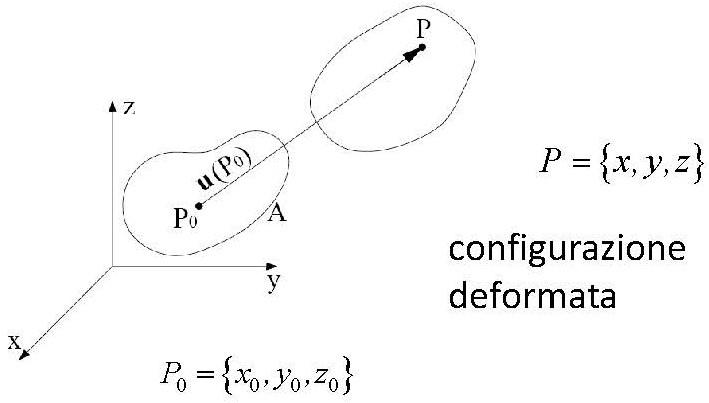
\includegraphics[width=0.4\linewidth]{immagini/1.PARTE7_Pagina_22 (2)}
\end{figure}
	Si indichino le componenti cartesiano del campo di spostamenti del punto P come:
	\[
	\begin{array}{c}
		u = u_x = x - x_0 \\
		v = u_y = y - y_0 \\
		w = u_z = z - z_0
	\end{array}
	\]
		Per descrivere lo stato di deformazione del corpo non ci si può più limitare a questi spostamenti ma sarà necessario introdurre una serie di riferimenti lineari, ortogonali tra loro, ovvero una terna di elementi lineari $dx, dy, dz$ solidali a $P_0$, che nella configurazione deformata si trasformi in $dL_x, dL_y, dL_z$ dove ogni elemento modifica la sua lunghezza e il suo angolo relativo.
\begin{figure}[H]
	\centering
	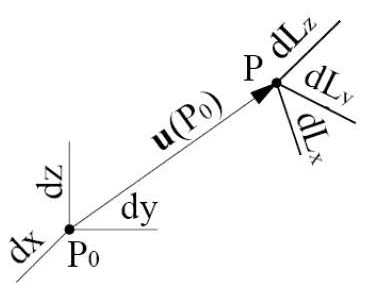
\includegraphics[width=0.25\linewidth]{immagini/1.PARTE7_Pagina_22}
\end{figure}
	Ci si chiede perciò, a seguito della deformazione, come varia la terna assegnata? \newline 
	
	Si impone per semplicità di trattazione che gli spostamenti rimangano al piano di appartenenza, ovvero sul piano $xy$.
	
\begin{figure}[H]
	\centering
	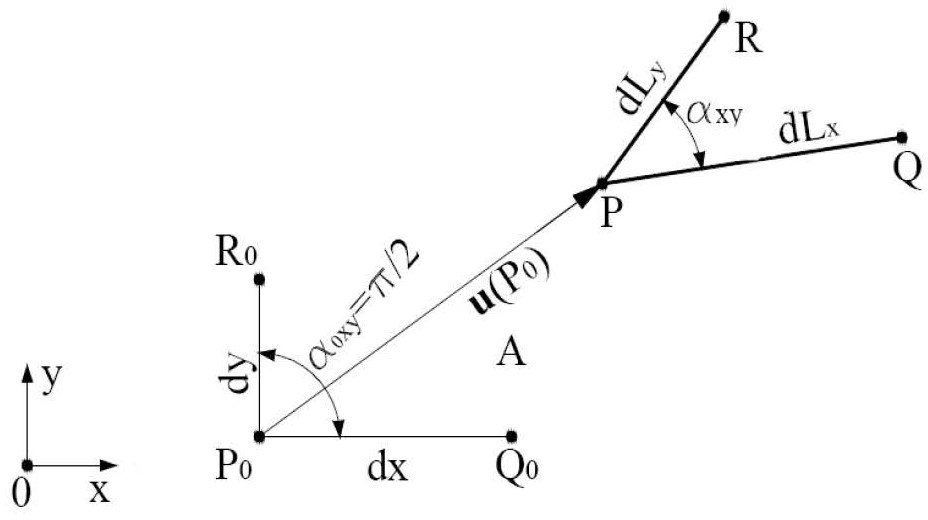
\includegraphics[width=0.4\linewidth]{immagini/1.PARTE7_Pagina_23}
\end{figure}
	A seguito di queste azioni si avranno allora una serie di
\begin{itemize}
		\item dilatazioni lineari, ovvero variazioni di lunghezza del tratto considerato: 
	\[\begin{cases}		
	\varepsilon_{xx} = \frac{PQ-P_0Q_0}{P_0Q_0} \\	
	\varepsilon_{yy} = \frac{PR-P_0R_0}{P_0R_0} \\	
  	\varepsilon_{zz} = \frac{PS-P_0S_0}{P_0S_0} \\
	\end{cases}
  	\]
	\item scorrimenti angolari o distorsioni: 
	\[\begin{cases}		
	\gamma_{xy} = \alpha_{0xy} - \alpha_{xy}\\
	\gamma_{xz} = \alpha_{0xz} - \alpha_{xz}\\
	\gamma_{yz} = \alpha_{0yz} - \alpha_{yz}
	\end{cases}
	\]
	Dove la condizione: 
	\[ \alpha_{0xy} + \alpha_{0xz} + \alpha_{0yz} = \frac{\pi}{2}
	\]
	È null'altro che la condizione di partenza, indeformata, con gli assi ortogonali tra loro.
\end{itemize}
	Queste osservazioni  sulle deformazioni vanno riportate in funzione del campo di spostamenti: ci si chiede, qual è lo stato deformativo che si instaura in base ad un determinato campo di spostamenti e viceversa? Per poter scrivere questo nella maniera più semplice deve continuare a valere l'ipotesi per cui la configurazione deformata sia molto "vicina" a quella indeformata, e dunque gli spostamenti sono infinitesimi, sono in questo modo è possibile ottenere una relazione lineare tra spostamenti e dilatazioni. 
	
	Sempre nell'ambito della teoria lineare si trascureranno poi tutti i termini del secondo ordine. 
	
\newpage
	
	È possibile scrivere allora per ciascun punto uno spostamento nella propria direzione.
	
\begin{figure}[H]
	\centering
	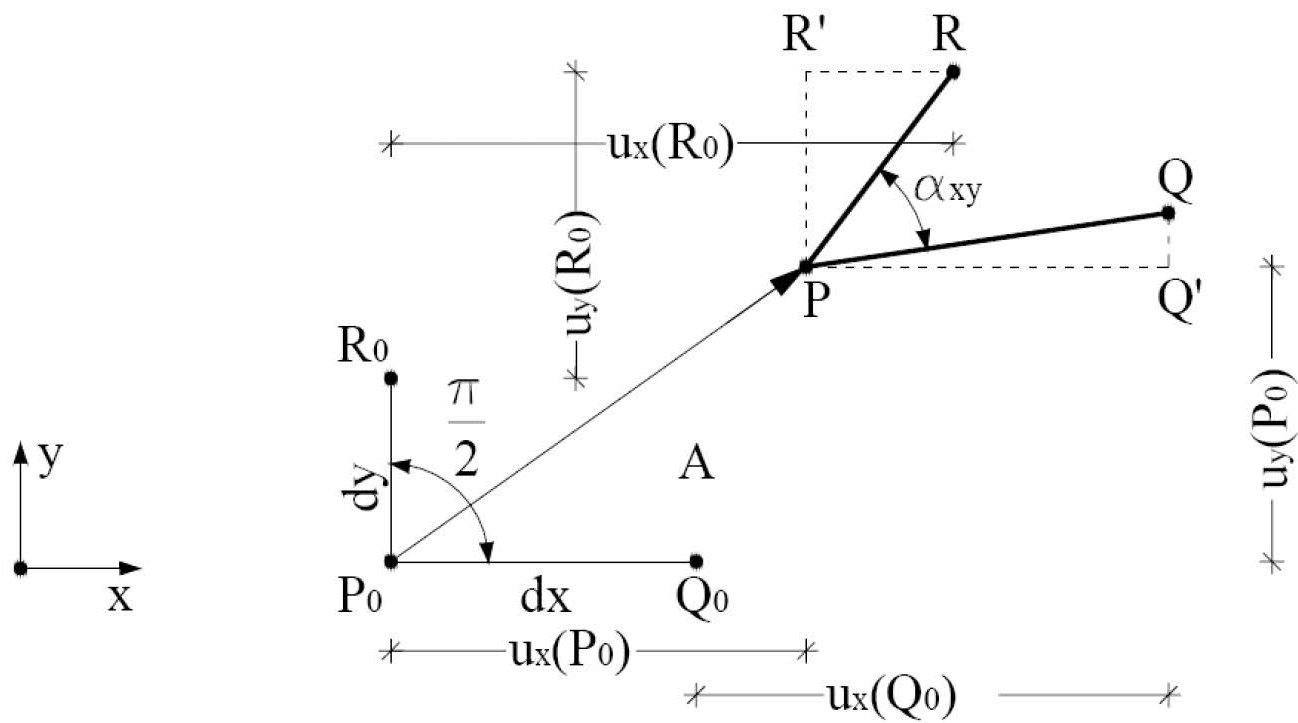
\includegraphics[width=0.5\linewidth]{immagini/1.PARTE7_Pagina_24}
\end{figure}
	Data una funzione $u_x$ che descriva gli spostamenti compresi tra $P_0$ e $Q_0$, lo spostamento di $Q_0$ è dato dallo spostamento di $P_0$ più la variazione che questa legge $u_x$ subisce muovendosi da $P_0$ a $Q_0$.
	 
	\[
	\begin{cases}
		u_x(Q_0) = u_x(x+dx, y, z) = u_x(P_0) + \left( \frac{\partial u_x}{\partial x}\right)_{P_0}dx\\
	u_y(Q_0) = u_y(x+dx, y, z) = u_y(P_0) + \left( \frac{\partial u_y}{\partial x}\right)_{P_0}dx\\
	u_x(R_0) = u_x(x, y+dy, z) = u_x(P_0) + \left( \frac{\partial u_x}{\partial y}\right)_{P_0}dy\\
	u_y(R_0) = u_y(x, y+dy, z) = u_y(P_0) + \left( \frac{\partial u_y}{\partial y}\right)_{P_0}dy
	\end{cases}
	\]
	I termini $\left( \frac{\partial u_x}{\partial x}\right)_{P_0}dx$ sono nient'altro che la possibile variazione di spostamento dei punti compresi  tra $P_0$ e $Q_0$ nella distanza $dx$.
	
	Per cui:
	\[
	PQ'= dL_x \approx  dx + u_x(Q_0) - u_x(P_0) = dx + \left( \frac{\partial u_x}{\partial x} \right)_{P_0}dy 	
	\]
	Questo risultato risponde alla domanda: quant'è lungo il lato $dx$ dopo la deformazione?
	
	Questo risultato è proprio la lunghezza finale del tratto $dx$. \newline
	
	Equivalentemente per le distorsioni si può scrivere:
	\[
	\begin{split}
			\alpha_{0xy} - \alpha_{xy} & = \frac{\pi}{2} - \alpha_{xy} = \hat{Q'PQ} + \hat{RPR'} = \overset{\text{arco/raggio}}{{QQ'\over dx} + {RR'\over dy}} = \\
			& = \frac{|u_y(Q_0) - u_y(P_0)|}{dx} + \frac{|u_x(R_0) - u_x(P_0)|}{dy} = \\
			& = \left( \frac{\partial u_y}{\partial x}\right)_{P_0} + \left( \frac{\partial u_x}{\partial y}\right)_{P_0}
	\end{split}
	\]
	In definitiva si può scrivere che la dilatazione lineare lungo $x$ ha la seguente forma:
	\[ \varepsilon_{xx} = \frac{dL_x - dx}{dx} = \left( \frac{\partial u_x}{\partial x}\right)_{P_0} \]
	E la distorsione dell'angolo retto $\alpha_{0xy}$ ha la seguente forma:
	\[\gamma_{xy} = \frac{\pi}{2} - \alpha_{xy} = \left( \frac{\partial u_y}{\partial x}\right)_{P_0} + \left( \frac{\partial u_x}{\partial y}\right)_{P_0}\]
\newpage	
	Attraverso un analogo procedimento per le altre direzioni, si ottengono infine le \newline 
	
	\begin{center}
		\textbf{Relazioni implicite di congruenza tra deformazioni e spostamenti associate ad uno Stato di deformazione del I ordine} \newline
	\end{center}
	
	Associati ovvero a piccoli spostamenti e piccole deformazioni.
	\[
	\begin{cases}
		\begin{aligned}
			\varepsilon_{xx} =  \left( \frac{\partial u_x}{\partial x}\right) \\
			\varepsilon_{yy} =  \left( \frac{\partial u_y}{\partial y}\right) \\
			\varepsilon_{zz} =  \left( \frac{\partial u_z}{\partial z}\right) \\
		\end{aligned}
	\end{cases} \hspace{1cm} \begin{cases}
		\begin{aligned}
			\gamma_{xy} =   \left( \frac{\partial u_y}{\partial x}\right) + \left( \frac{\partial u_x}{\partial y}\right) \\
			\gamma_{yz} =   \left( \frac{\partial u_y}{\partial z}\right) + \left( \frac{\partial u_z}{\partial y}\right) \\
			\gamma_{zx} =   \left( \frac{\partial u_z}{\partial x}\right) + \left( \frac{\partial u_x}{\partial z}\right) \\
		\end{aligned}
	\end{cases} \hspace{1cm} \begin{cases}
	\begin{aligned}
		\gamma_{xy} =   \gamma_{yx} \\
		\gamma_{yz} =   \gamma_{zy} \\
		\gamma_{zx} =   \gamma_{xz} \\
	\end{aligned}
	\end{cases}
	\]
	Dove le dilatazioni e le distorsioni sono rispettivamente le derivate parziali e le derivate parziali incrociate degli spostamenti. \newline 
	
	In forma matriciale: 
	\[
	u(Q) = u(P) + du
	\]
	\[
	du = [du_x, du_y, du_z]~\text{variazione di spostamento}
	\]
	\[
	du_x = \frac{\partial u_x}{\partial x} dx + \frac{\partial u_x}{\partial y}dy + \frac{\partial u_x}{\partial z}dz
	\]
	\[
	du_y = \frac{\partial u_y}{\partial x} dx + \frac{\partial u_y}{\partial y}dy + \frac{\partial u_y}{\partial z}dz
	\]
	\[
	du_z = \frac{\partial u_z}{\partial x} dx + \frac{\partial u_z}{\partial y}dy + \frac{\partial u_z}{\partial z}dz
	\]
	\[
		\left[ \begin{array}{c}
			u_x(Q) \\
			u_y(Q) \\
			u_z(Q)
		\end{array}\right] = \left[ \begin{array}{c}
		u_x(P) \\
		u_y(P) \\
		u_z(P)
	\end{array}\right] + \left[\begin{array}{ccc}
	
	\dfrac{\partial u_x}{\partial x} & \dfrac{\partial u_x}{\partial y} & \dfrac{\partial u_x}{\partial z} \\ 
	\dfrac{\partial u_y}{\partial x} & \dfrac{\partial u_y}{\partial y} & \dfrac{\partial u_y}{\partial z} \\ 
	\dfrac{\partial u_z}{\partial x} & \dfrac{\partial u_z}{\partial y} & \dfrac{\partial u_z}{\partial z}
		
	\end{array} \right] \left[ \begin{array}{c}
		dx \\
		dy \\
		dz
	\end{array}\right] 
	\]
	Si disaccoppia a questo punto il campo di spostamenti complessivo in uno deformativo $E$ e in un altro rototraslatorio $\Omega$, allora la matrice F sarà somma di una componente simmetrica $E$ e di una antisimmetrica $\Omega$:	
	\[
	F = \left[\begin{array}{ccc}
		
		\dfrac{\partial u_x}{\partial x} & \dfrac{\partial u_x}{\partial y} & \dfrac{\partial u_x}{\partial z} \\ 
		\dfrac{\partial u_y}{\partial x} & \dfrac{\partial u_y}{\partial y} & \dfrac{\partial u_y}{\partial z} \\ 
		\dfrac{\partial u_z}{\partial x} & \dfrac{\partial u_z}{\partial y} & \dfrac{\partial u_z}{\partial z}
		
	\end{array} \right] = E + \Omega
	\]
	\vspace{1cm}
	\[
	E = \frac{1}{2} [F + F^T] 
	\]
	\[
	\Omega = \frac{1}{2} [F - F^T] 
	\]
	\vspace{1cm}
	\[
	E = \left[\begin{array}{ccc}
		
		\dfrac{\partial u_x}{\partial x} & \dfrac{1}{2}\left( \dfrac{\partial u_x}{\partial y} + \dfrac{\partial u_y}{\partial x} \right)  & \dfrac{1}{2}\left( \dfrac{\partial u_x}{\partial z} + \dfrac{\partial u_z}{\partial x}\right) \\ 
		\dfrac{1}{2}\left(\dfrac{\partial u_y}{\partial x} + \dfrac{\partial u_x}{\partial y} \right) & \dfrac{\partial u_y}{\partial y} & \dfrac{1}{2}\left(\dfrac{\partial u_y}{\partial z} + \dfrac{\partial u_z}{\partial y} \right) \\ 
		\dfrac{1}{2}\left(\dfrac{\partial u_z}{\partial x} +\dfrac{\partial u_x}{\partial z} \right)  & \dfrac{1}{2}\left(\dfrac{\partial u_z}{\partial y} + \dfrac{\partial u_y}{\partial z}\right)  & \dfrac{\partial u_z}{\partial z}
		
	\end{array} \right]
	\]	
	\vspace{1cm}
	\[
	\Omega = \left[\begin{array}{ccc}		
		0 & \dfrac{1}{2}\left( \dfrac{\partial u_x}{\partial y} - \dfrac{\partial u_y}{\partial x} \right)  & \dfrac{1}{2}\left( \dfrac{\partial u_x}{\partial z} - \dfrac{\partial u_z}{\partial x}\right) \\ 
		\dfrac{1}{2}\left(\dfrac{\partial u_y}{\partial x} - \dfrac{\partial u_x}{\partial y} \right) & 0 & \dfrac{1}{2}\left(\dfrac{\partial u_y}{\partial z} - \dfrac{\partial u_z}{\partial y} \right) \\ 
		\dfrac{1}{2}\left(\dfrac{\partial u_z}{\partial x} -\dfrac{\partial u_x}{\partial z} \right)  & \dfrac{1}{2}\left(\dfrac{\partial u_z}{\partial y} - \dfrac{\partial u_y}{\partial z}\right)  & 0		
	\end{array} \right]
	\] 
	La matrice $E$ è anche conosciuta come Tensore di Cauchy ed è legato alle deformazioni: 
	\[
	E = \left[ \begin{array}{ccc}
		\varepsilon_{xx} & \varepsilon_{xy} & \varepsilon_{xz} \\
		\varepsilon_{yx} & \varepsilon_{yy} & \varepsilon_{yz} \\
		\varepsilon_{zx} & \varepsilon_{zy} & \varepsilon_{zz}
	\end{array} \right] 
	\]
	Le componenti del tensore di Cauchy divengono così pari a:
	\[
	\begin{cases}
		\begin{aligned}
			\varepsilon_{xx} =  \frac{1}{2}\left( \frac{\partial u_x}{\partial x} + \frac{\partial u_x}{\partial x} \right) \\
			\varepsilon_{yy} =  \frac{1}{2}\left( \frac{\partial u_y}{\partial y} + \frac{\partial u_y}{\partial y}\right) \\
			\varepsilon_{zz} =  \frac{1}{2}\left( \frac{\partial u_z}{\partial z} + \frac{\partial u_z}{\partial z}\right) \\
		\end{aligned}
	\end{cases} \hspace{1cm} \begin{cases}
	\begin{aligned}
		\varepsilon_{xy} =  \frac{\gamma_{xy}}{2} = \frac{1}{2}\left( \frac{\partial u_y}{\partial x} + \frac{\partial u_x}{\partial y} \right) \\
		\varepsilon_{yz} =  \frac{\gamma_{yz}}{2} = \frac{1}{2}\left( \frac{\partial u_y}{\partial z} + \frac{\partial u_z}{\partial y}\right) \\
		\varepsilon_{zx} =  \frac{\gamma_{zx}}{2} = \frac{1}{2}\left( \frac{\partial u_z}{\partial x} + \frac{\partial u_x}{\partial z}\right) \\
	\end{aligned}
\end{cases}
	\]
	Si può definire anche qui una terna principale, ovvero una terna rispetto alla quale gli elementi lineari non subiscano distorsioni ma solo dilatazioni, in questo modo il tensore di Cauchy possiede solo la diagonale. \newline
	
	Se si ha a che fare con un corpo isotropo, ovvero con un materiale dal comportamento uniforme rispetto a tutte le direzioni possibili, allora le direzioni principali delle tensioni equivalgono alle direzioni principali delle deformazioni. \newline  
	
	Dato un campo di spostamenti ad esso corrisponde uno stato di
	deformazione, infatti svolgendo le derivate parziali degli spostamenti si ottiene sempre un campo di deformazioni, mentre il contrario non è sempre vero, ovvero ad un campo di deformazioni non corrisponde necessariamente un campo di
	spostamenti che sia compatibile, infatti il sistema di equazioni differenziali proposto non è sempre integrabile, questo significa dire in pratica che, associati a determinati campi di deformazione si possono avere campi di spostamento che generino separazioni o compenetrazioni di materiale. \newline 
	
	Il rispetto della compatibilità avviene mediante le relazioni di compatibiltià, queste permettono infatti di comprendere se un campo di deformazioni genera un campo di spostamenti compatibile. \newline
	
	Si consideri allora un corpo come un insieme di volumi infinitesimi la cui deformazione
	è dettata, nell’intorno infinitesimo di un punto, dalle derivate precedentemente introdotte.
	
	Il loro valore non potrà essere arbitrario e indipendente, ma dovrà essere
	compatibile con i volumi adiacenti per non generare compenetrazioni o
	separazioni.

	Le condizioni di integrabilità sono state espresse da Saint
	Venant e Beltrami e
	sono denominate \textbf{equazioni esplicite di compatibilità o congruenza}.

\begin{figure}[H]
	\centering
	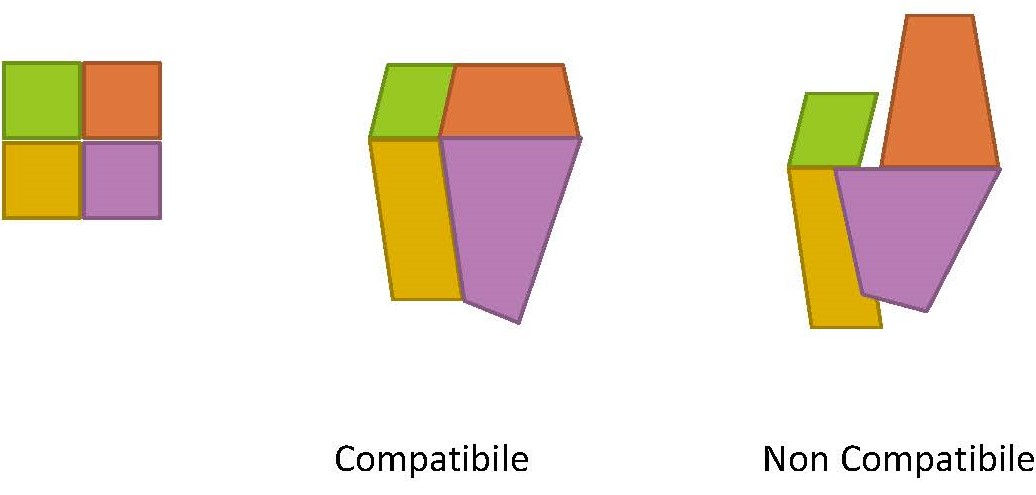
\includegraphics[width=0.4\linewidth]{immagini/1.PARTE7_Pagina_31}
\end{figure}

	La forma esplicita di queste equazioni di compatibilità non saranno trattate, ai fini del corso basta far rispettare quelle del primo ordine, ma è importante capire che l'applicazione delle equazioni di congruenza permette di mettersi al riparo dalla presenza di spostamenti che generino separazione o compenetrazioni di materiale. \newline 

{\Large \textbf{Legame Costitutivo I}} \newline 

	Si è impostato il problema elastico	attraverso le equazioni di equilibrio sul volume e sul contorno, alle quali si è associato il legame di compatibilità tra spostamenti e deformazioni affinché esistano spostamenti compatibili, manca ancora però da definire il legame che intercorre tra lo stato tensionale e quello deformativo. \newline 
	
	Perché sarà proprio il comportamento del materiale a definire lo stato tensionale che scaturisce da una determinata deformazione e viceversa. \newline
	
	Si tratta di definire delle equazioni costitutive che leghino tensioni e deformazioni e
	caratterizzino il materiale del corpo. 
	
	Il legame costitutivo che si andrà ad individuare è proprio del tipo di materiale che si andrà a considerare. \newline 

	Esiste quindi un termine che lega nel tempo il campo di deformazioni alle tensioni che si instaurano punto per punto. \newline 

	Il comportamento ideale dei materiali esistenti è stato catalogato attraverso le curve caratteristiche: 
	\begin{itemize}
		\item Elastico
		\item Plastico
		\item Viscoso
		\item Elasto plastico
		\item Visco plastico
		\item \dots
	\end{itemize}

	\[ \sigma_{ij} = f(\varepsilon_{hk}, t)\]
	
	Ci si occupi, per ora, del solo comportamento elastico lineare, per cui si ignora ogni qualsiasi
	influenza della «storia» precedente di carico: elasticità del I ordine. \newline 
	
	Ci si ponga nelle ipotesi di materiale isotropo: il suo comportamento non dipende dalla direzione
	di sollecitazione.\newline
	
	Ci si ponga nelle ipotesi di materiale omogeneo: le grandezze caratteristiche del materiale sono
	uniformi, riscontrabili identiche a sè stesse in qualunque punto del materiale. \newline 
	
	Allora il \textbf{legame costitutivo di Navier} prende la seguente forma:	
		\[
	\begin{cases}
		\begin{aligned}
			\varepsilon_{xx} =  \frac{1}{E}\left[ \sigma_x - \nu(\sigma_y + \sigma_z) \right] \\
			\varepsilon_{yy} =  \frac{1}{E}\left[ \sigma_y - \nu(\sigma_x + \sigma_z) \right] \\
			\varepsilon_{zz} =  \frac{1}{E}\left[ \sigma_z - \nu(\sigma_x + \sigma_y) \right] \\
		\end{aligned}
	\end{cases} \hspace{1cm} \begin{cases}
		\begin{aligned}
			\varepsilon_{xy} =  \frac{\tau_{xy}}{2G} \\
			\varepsilon_{yz} =  \frac{\tau_{yz}}{2G} \\
			\varepsilon_{zx} =  \frac{\tau_{zx}}{2G}  \\
		\end{aligned}
	\end{cases}
	\]
	Dove si definiscono : 
	\begin{itemize}
	\item Modulo elastico tangenziale 
	\[ G = \frac{E}{2(1+ \nu)} \]
	
	\item Modulo di Young o Elasticità normale
	 \[E > 0\]

 	\item Coefficiente di Poisson 
 	\[-1<\nu<0.5\]
 	Variabile a seconda del comportamento del materiale.
	\end{itemize}
	In cui solo de sono indipendenti, solitamente si definiscono $E, \nu$ e poi si ricava $G$. \newline 
	
	La forma matriciale delle equazioni di Navier, mettendo in relazione i termini del tensore di Cauchy con quelli del tensore delle tensioni diviene:
	\[
	\left[\begin{array}{c}
		\varepsilon_{xx} \\
		\varepsilon_{yy} \\
		\varepsilon_{zz} \\
		\varepsilon_{xy} \\
		\varepsilon_{yz} \\
		\varepsilon_{xz}
	\end{array} \right] = \frac{1}{E} \left[ \begin{array}{cccccc}
			1 & -\nu & -\nu & 0 & 0 & 0 \\
			-\nu & 1 & -\nu & 0 & 0 & 0 \\
			-\nu & -\nu & 1 & 0 & 0 & 0 \\
			0 & 0 & 0 & 1 + \nu & 0 & 0 \\
			0 & 0 & 0 & 0 & 1 + \nu & 0 \\
			0 & 0 & 0 & 0 & 0 & 1 + \nu
	\end{array}\right] \left[ \begin{array}{c}
		\sigma_{xx} \\
		\sigma_{yy} \\
		\sigma_{zz} \\
		\tau_{xy} \\
		\tau_{yz} \\
		\tau_{xz}
	\end{array} \right] 
	\]

	E dunque	
	
	\[
	\left[ \begin{array}{c}
		\sigma_{xx} \\
		\sigma_{yy} \\
		\sigma_{zz} \\
		\tau_{xy} \\
		\tau_{yz} \\
		\tau_{xz}
	\end{array} \right]  = \frac{E}{(1+\nu)(1-2\nu)} \left[ \begin{array}{cccccc}
		1 -\nu & \nu & \nu & 0 & 0 & 0 \\
		\nu & 1 -\nu & \nu & 0 & 0 & 0 \\
		\nu & \nu & 1 -\nu & 0 & 0 & 0 \\
		0 & 0 & 0 & \dfrac{1 + 2\nu}{2} & 0 & 0 \\
		0 & 0 & 0 & 0 & \dfrac{1 + 2\nu}{2} & 0 \\
		0 & 0 & 0 & 0 & 0 & \dfrac{1 + 2\nu}{2}
	\end{array}\right] \left[\begin{array}{c}
		\varepsilon_{xx} \\
		\varepsilon_{yy} \\
		\varepsilon_{zz} \\
		2\varepsilon_{xy} \\
		2\varepsilon_{yz} \\
		2\varepsilon_{xz}
	\end{array} \right]
	\]

Nel caso di \textbf{Stato di Tensione Piano}: $ \sigma_z - \tau_{xz} = \tau_{yz} = 0 \Rightarrow \varepsilon_{zz} = 0$ la deformazione in $z$ non è nulla, ma è legata agli effetti di strizione in $\sigma_x$ e $\sigma_y$.
	\[
	\left[\begin{array}{c}
		\varepsilon_{xx} \\
		\varepsilon_{yy} \\
		\varepsilon_{zz} \\
		\varepsilon_{xy} \\
	\end{array} \right] = \frac{1}{E} \left[ \begin{array}{ccc}
		1 & -\nu & 0 \\
		-\nu & 1 & 0 \\
		-\nu & -\nu & 0\\
		0 & 0  & 1 + \nu 
	\end{array}\right] \left[ \begin{array}{c}
		\sigma_{xx} \\
		\sigma_{yy} \\
		\tau_{xy} \\
	\end{array} \right] 
	\]

	La matrice di rigidezza associa uno stato di tensione piano ad uno stato di tensione tridimensionale.  
\newpage	
	La $\varepsilon_{zz}$ può anche non essere definita esplicitamente perché è combinazione lineare.  

	\[
	  \left[ \begin{array}{c}
 		\sigma_{xx} \\
 		\sigma_{yy} \\
 		\tau_{xy} \\
 	\end{array} \right] = \frac{E}{1-\nu^2} \left[ \begin{array}{ccc}
			1 & \nu & 0 \\
			\nu & 1 & 0 \\
			-\nu & -\nu & 0\\
			0 & 0  & \dfrac{1 - \nu}{2} 
	\end{array}\right] \left[\begin{array}{c}
		\varepsilon_{xx} \\
		\varepsilon_{yy} \\
		2\varepsilon_{xy} \\
	\end{array} \right] 
	\]
	Lo stato di deformazione è tridimensionale: $\varepsilon_{xz} = \varepsilon_{yz}=0$ \newline 

Analogamente, uno \textbf{stato di deformazione piano}: $ \varepsilon_{zz} = \varepsilon_{xz} = \varepsilon_{yz} = 0$ comporta $\sigma_{zz} \ne 0$ in quanto queste saranno generate dai contributi delle $\varepsilon_{xx}, \varepsilon_{yy}$.

	\[
	\left[ \begin{array}{c}
		\sigma_{xx} \\
		\sigma_{yy} \\
		\sigma_{zz} \\
		\tau_{xy} \\
	\end{array} \right] = \frac{E}{(1+\nu)(1-2\nu)} \left[ \begin{array}{ccc}
		1 - \nu & \nu & 0 \\
		\nu & 	1 - \nu & 0 \\
		\nu & \nu & 0\\
		0 & 0  & \dfrac{1 - 2\nu}{2} 
	\end{array}\right] \left[\begin{array}{c}
		\varepsilon_{xx} \\
		\varepsilon_{yy} \\
		2\varepsilon_{xy} \\
	\end{array} \right] 
	\]	
	Dove anche qui la terza equazione è combinazione lineare delle precedenti due, quindi non necessaria. \newline 

	Lo stato di tensione è tridimensionale. 

\begin{figure}[H]
	\centering
	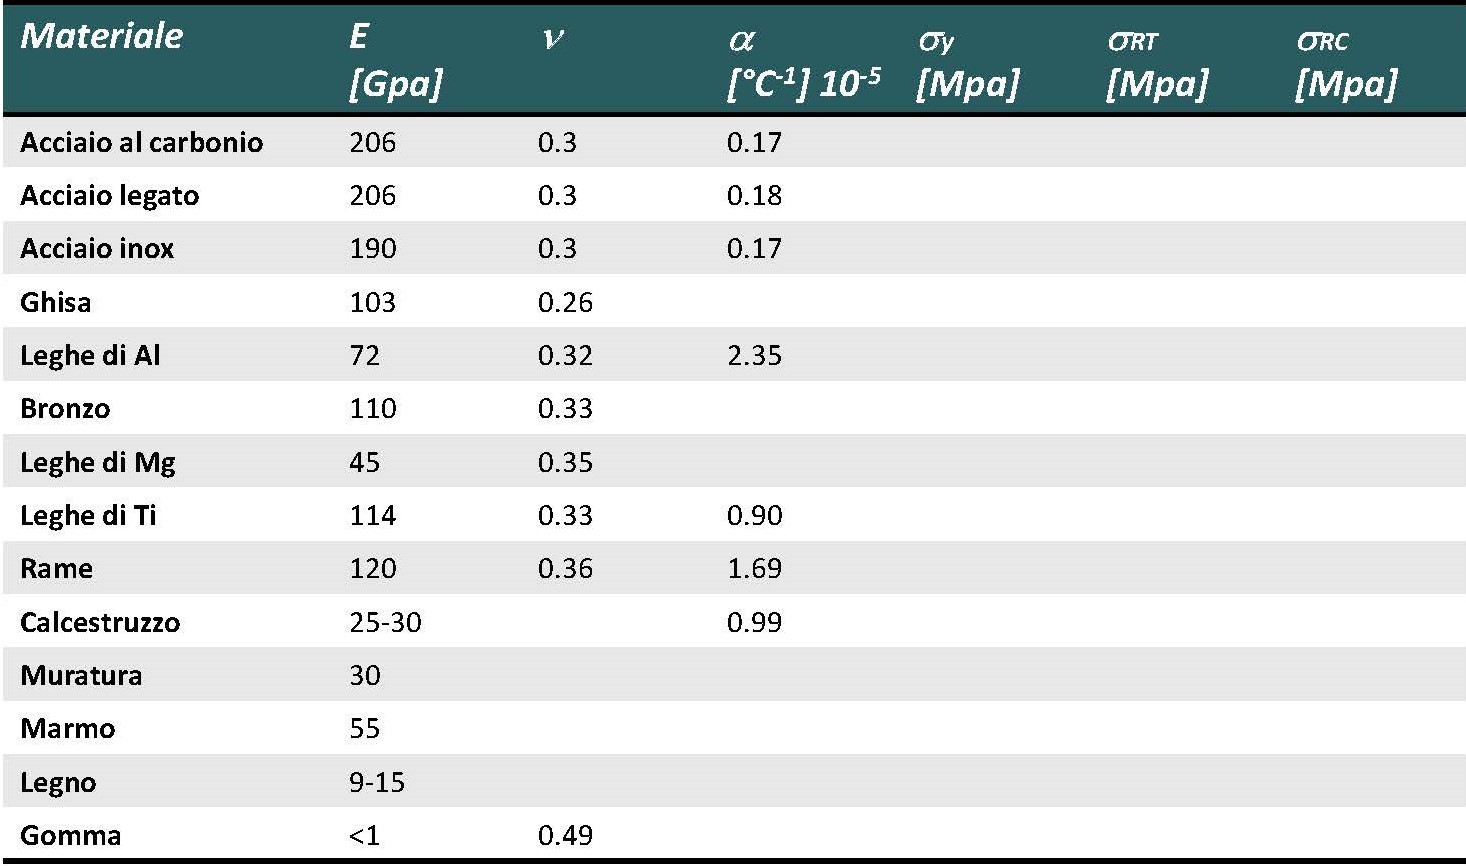
\includegraphics[width=0.8\linewidth]{immagini/1.PARTE7_Pagina_37}
\end{figure} 
\newpage


{\Large \textbf{Circonferenze di Mohr}} \newline 	
	Un modo per diagrammare lo stato tensionale ma anche lo stato deformativo al variare della giacitura rispetto alle quali si esprimono tali grandezze passa attraverso le circonferenze di Mohr. \newline 
	
	Le circonferenze di Mohr rappresentano i possibili valori dello stato tensionale secondo un fascio di piani avente per sostegno un asse coincidente con una direzione principale. \newline 
	
	Con le circonferenze di Mohr si va a rappresentare lo stato tensionale in un punto rispetto ad un set di assi di riferimento, questi si scelgono a partire da fasci di piani aventi tutti in comune una direzione principale. 	\newline 
	
	Esse sono una rappresentazione bidimensionale dello stato di tensione tridimensionale in un
	punto P. \newline
	
	Tale rappresentazione non ha senso se non è nota almeno una delle direzioni principali. \newline
	
	HP: $\tau_{xz} = \tau_{yz} = 0; \forall \sigma_z $ \newline
	
	Si immagini di conoscere una terna principale $x,y,z$ e si interrompa un volume materiale infinitesimo con un piano $\alpha$, nasceranno allora tensioni $\sigma$ e $\tau$. 
	
\begin{figure}[H]
	\centering
	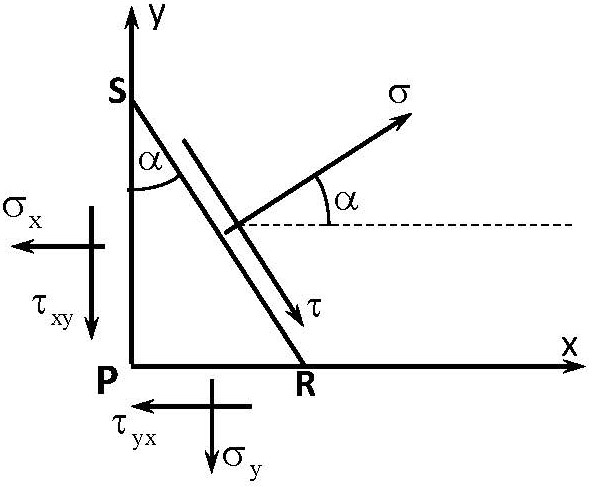
\includegraphics[width=0.4\linewidth]{immagini/1.PARTE7_Pagina_38}
\end{figure} 

	Ipotizzando $\alpha$ noto, varranno le seguenti relazioni. 
	
	\[
	\begin{cases}
		\overline{PS} = \overline{RS} \cos\alpha\\
	\overline{PR} = \overline{RS} \sin\alpha
	\end{cases}
	\]
	Si assuma momento orario per $ \tau > 0 $
	
	In questo modo le rotazioni nel
	riferimento geometrico e
	nel piano di Mohr avranno lo
	stesso verso. \newline 
	
	Imponendo l'equilibrio a traslazione in direzione $\sigma$ e $\tau$ e semplificando $\overline{SR}dz$, si ottiene
	\[
	\begin{split}
		\sigma(\alpha) & = \sigma_x \cos^2 \alpha + \sigma_y \sin^2 \alpha + 2\tau_{xy} \sin\alpha \cos\alpha = \\
					   & = \sigma_x\left( \frac{1+ \cos2\alpha}{2}\right)  + \sigma_y \left( \frac{1- \cos2\alpha}{2}\right) + \tau_{xy} \sin2\alpha = \\
					   & = \frac{1}{2} (\sigma_x + \sigma_y) + \frac{1}{2}  (\sigma_x + \sigma_y) \cos2\alpha + \tau_{xy} \sin2\alpha
	\end{split}
	\]
	Dove sono state sfruttate le formule di bisezione dell'angolo e si sono raccolti tutti i termini $\sigma_x, \sigma_y, \tau_{xy}$. 
	
	Similmente:
	\[
	\begin{split}
		\tau(\alpha) & = \sigma_x \sin\alpha\cos\alpha - \sigma_y \sin\alpha\cos\alpha + \tau_{yx} \sin^2\alpha - \tau_{xy} \cos^2\alpha = \\
					   & = -\tau_{xy} \cos2\alpha + \frac{1}{2} (\sigma_x - \sigma_y) \sin2\alpha
	\end{split}
	\]
	
	Sotto le ipotesi di $x,y,z$ terna principale, $\tau_{xy} = 0$, se poi $\sigma_x=\sigma_1$ e $\sigma_y=\sigma_2$ rimangono le equazioni
	parametriche di una circonferenza nel piano $\sigma\tau$: 
	
	\[
	\begin{cases}
		\begin{aligned}
	\sigma & = \frac{1}{2} (\sigma_1 + \sigma_2) + \frac{1}{2}  (\sigma_1 + \sigma_2) \cos2\alpha \\
	\tau & = \frac{1}{2} (\sigma_1 - \sigma_2) \sin2\alpha
		\end{aligned}
	\end{cases}
	\]
	
	Infatti posti 
	\begin{itemize}
	\item	\[\delta = \frac{1}{2} (\sigma_1 + \sigma_2)\]
	Spostamento del centro della circonferenza dall'origine
	
	\item \[\rho = \frac{1}{2} (\sigma_1 - \sigma_2)\]
	Raggio della circonferenza
	\end{itemize}
	Si ottiene:
	\[
	\begin{cases}
		\begin{aligned}
			\sigma - \delta & = \rho \cos2\alpha \\
			\tau & = \rho \sin2\alpha
		\end{aligned}
	\end{cases} \Rightarrow (\sigma - \delta)^2 + \tau^2 = \rho^2
	\]
	Se in un riferimento cartesiano al posto delle $x,y$  si utilizzano le $\sigma,\tau$ quello appena scritto è un sistema di equazioni che in un piano $\sigma,\tau$ restituisce una circonferenza. \newline
	
	Questo vuol dire che la rappresentazione di un punto sulla circonferenza di Mohr indica la rappresentazione dello stato tensionale quando si ruota il sistema di riferimento rispetto a delle direzioni principali di un angolo $\alpha$ intorno ad un asse principale. \newline
	
Se le tre direzioni principali davano $\sigma_1$, $\sigma_2$ (e $\sigma_3$), compiendo una rotazione di angolo $\alpha$  dalle direzioni principali, non si avrà più una configurazione principale, ma una configurazione che si popola di elementi fuori diagonale. \newline 

Se ad esempio nella direzione principale si aveva:
\[\left[ \begin{array}{ccc}
	\sigma_1 & 0 & 0 \\
	0 & \sigma_2 & 0 \\
	0 & 0 & 0 
\end{array}\right]\]
Ed è necessario conoscere le tensioni rispetto ad una terna generica, facendo ruotare la terna principale si ottiene una matrice lungo una direzione non più principale
\[\left[ \begin{array}{ccc}
	\sigma_1 & \tau_{xy} & 0 \\
	\tau_{xy} & \sigma_2 & 0 \\
	0 & 0 & 0 
\end{array}\right]\]

\textbf{NB:} Rotazioni di $2\alpha$ nel piano di Mohr corrispondono a rotazioni di $\alpha$ nel piano fisico.

\begin{figure}[H]
	\centering
	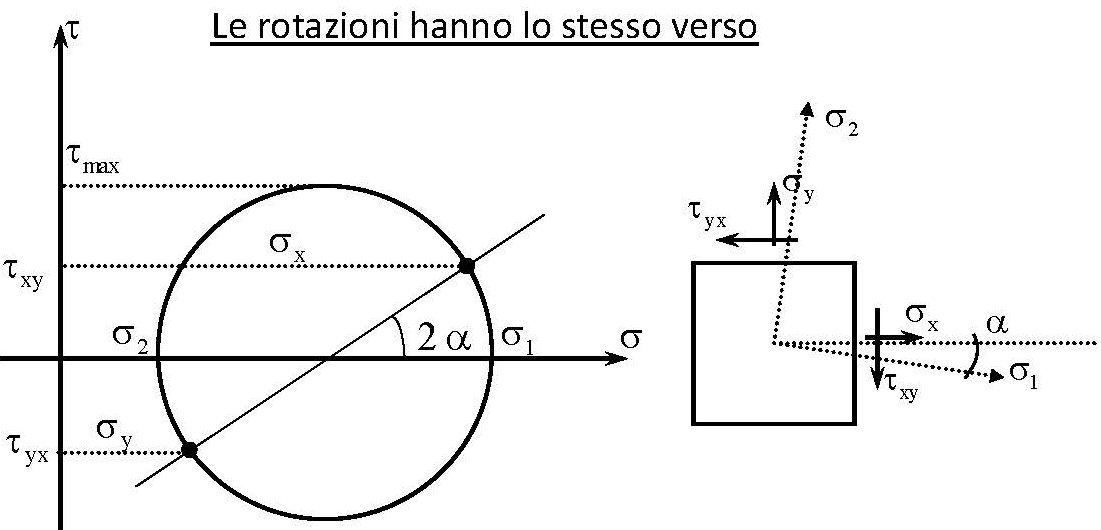
\includegraphics[width=0.7\linewidth]{immagini/1.PARTE7_Pagina_40}
\end{figure} 

Le coordinate in $x$ daranno così i valori di $\sigma_x$ e $\sigma_y$, mentre le coordinate in $y$ daranno le $\tau_{xy}$ e le $\tau_{yx}$. \newline 

	Questa rappresentazione permette di viaggiare facilmente tra coordinate/direzioni principali e non principali, infatti se si vuole conoscere l'angolo che si genera tra una direzione principale ed una direzione generica basta partire dalla stessa direzione generica e dai suoi valori di tensione, imporre la condizione $\tau = 0$ e risolvere in funzione di $\alpha$:

	\[
		\tau(\alpha) = -\tau_{xy} \cos2\alpha + \frac{1}{2}(\sigma_x -\sigma_y) \sin2\alpha \Rightarrow \begin{cases}
			\begin{aligned}
			\tan2\alpha & = \dfrac{2\tau_{xy}}{\sigma_x -\sigma_y} \\
			\alpha & = \dfrac{1}{2} \arctan \left(\dfrac{2\tau_{xy}}{\sigma_x -\sigma_y} \right) 
			\end{aligned}
		\end{cases}
	\]
	Il valore che ne scaturisce sarà l'angolo di rotazione necessario per passare da una terna generica ad una terna principale. \newline
	
	Al tempo stesso, attraverso Pitagora, si è in grado di calcolare anche i valori delle tensioni principali.
	
\begin{figure}[H]
	\centering
	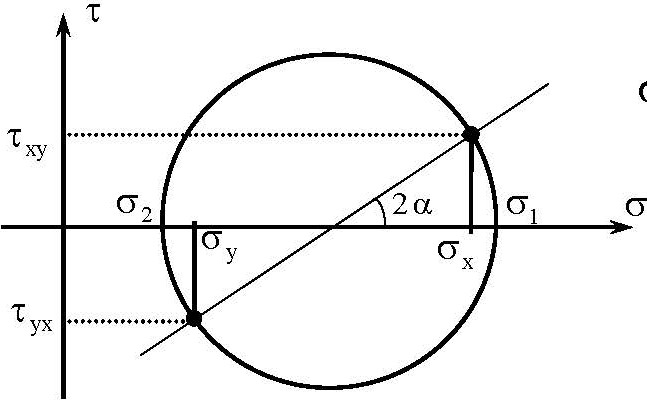
\includegraphics[width=0.4\linewidth]{immagini/1.PARTE7_Pagina_41}
\end{figure} 
	\[
	\sigma_{1,2} = \frac{\sigma_x + \sigma_y}{2} \pm \sqrt{\left( \frac{\sigma_x + \sigma_y}{2} \right)^2 + \tau_{xy}^2 }
	\]
	\newpage
	Quello che è stato fatto finora è stato tracciare la circonferenza $\sigma_1\sigma_2$, ovvero, data una terna principale $1,2,3$ è stato tenuto fuori $3$ e si sono compiute rotazioni $\alpha$ intorno ad esso, facendo ruotagli gli assi $1,2$ che diventano i generici $x,y$. 
	
	Allo stesso modo si potrebbe ripetere l'operazione facendo una rotazione intorno ad $1$ ottenendo così diverse rappresentazioni dello stato tensionale secondo terne non principali ma che hanno in comune un asse principale $\sigma_1$; oppure ancora far ruotare il piano di riferimento intorno all'asse $2$ rappresentando lo stato tensionale secondo terne sempre non principali ma aventi in comune l'asse $2$. 

\begin{figure}[H]
	\centering
	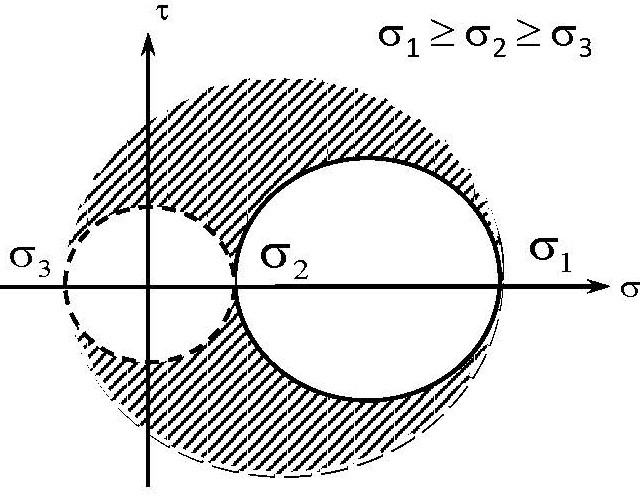
\includegraphics[width=0.4\linewidth]{immagini/1.PARTE7_Pagina_42 (2)}
\end{figure}	

	Questi tre cerchi di Mohr contengono nell'area tratteggiata tutte le possibili rappresentazioni dello stato tensionale in un punto: in una direzione non principale le
	tensioni si posizionano proprio nell’area
	tratteggiata, mentre i confini di quest'area descrivono la rappresentazione dello stato tensionale secondo terne in cui almeno un asse è principale. \newline 
	
	In base a come si dispongono queste circonferenze si può avere un'idea del tipo di stato tensionale che si ha in quel punto. \newline
	
	Si ricordi che Mohr è valido per un solo punto del corpo, questa è sostanzialmente una rappresentazione grafica dei valori che possono assumere i nove termini del tensore delle tensioni in un punto.
	
\begin{figure}[H]
	\centering
	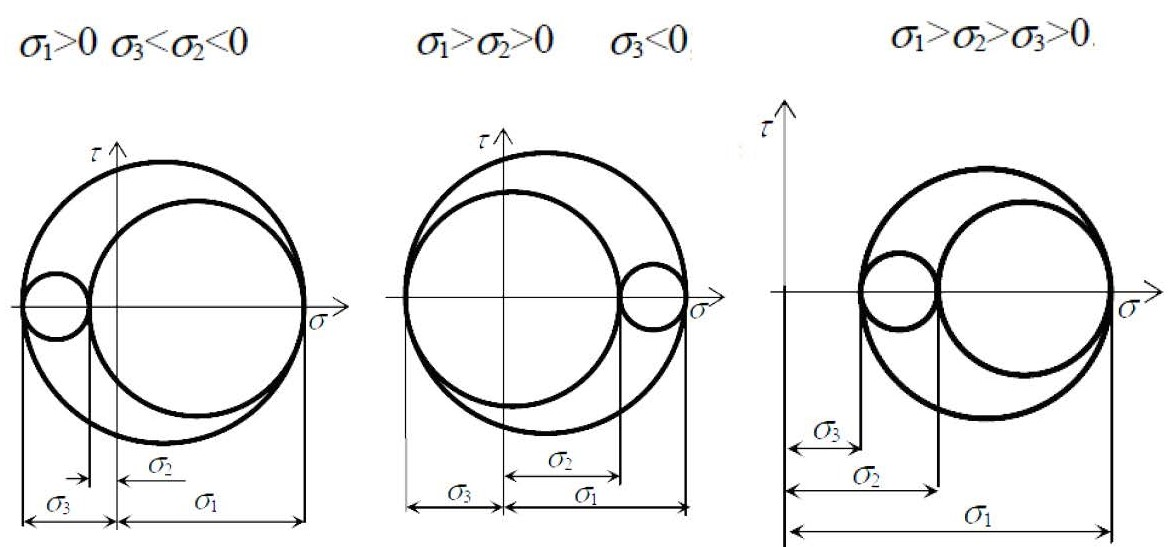
\includegraphics[width=0.8\linewidth]{immagini/1.PARTE7_Pagina_42}
\end{figure}
\newpage
	Nel caso di sollecitazione piana una delle tensioni principali è nulla per cui le circonferenze passeranno nell'origine. \newline 
	
	Nel caso di sollecitazione monodimensionale di sola trazione due tensioni principali sono nulle ed una è non nulla e positiva. 
	
	La rappresentazione delle 3 circonferenze consiste in due circonferenze sovrapposte $\sigma_1\sigma_2 + \sigma_2\sigma_2$  più una circonferenza degenere in un punto $\sigma_2\sigma_3$. \newline 
	
	In caso di sollecitazione monodimensionale di compressione, similmente a quella di trazione, due tensioni principali sono nulle ed una è non nulla e negativa.
\begin{figure}[H]
	\centering
	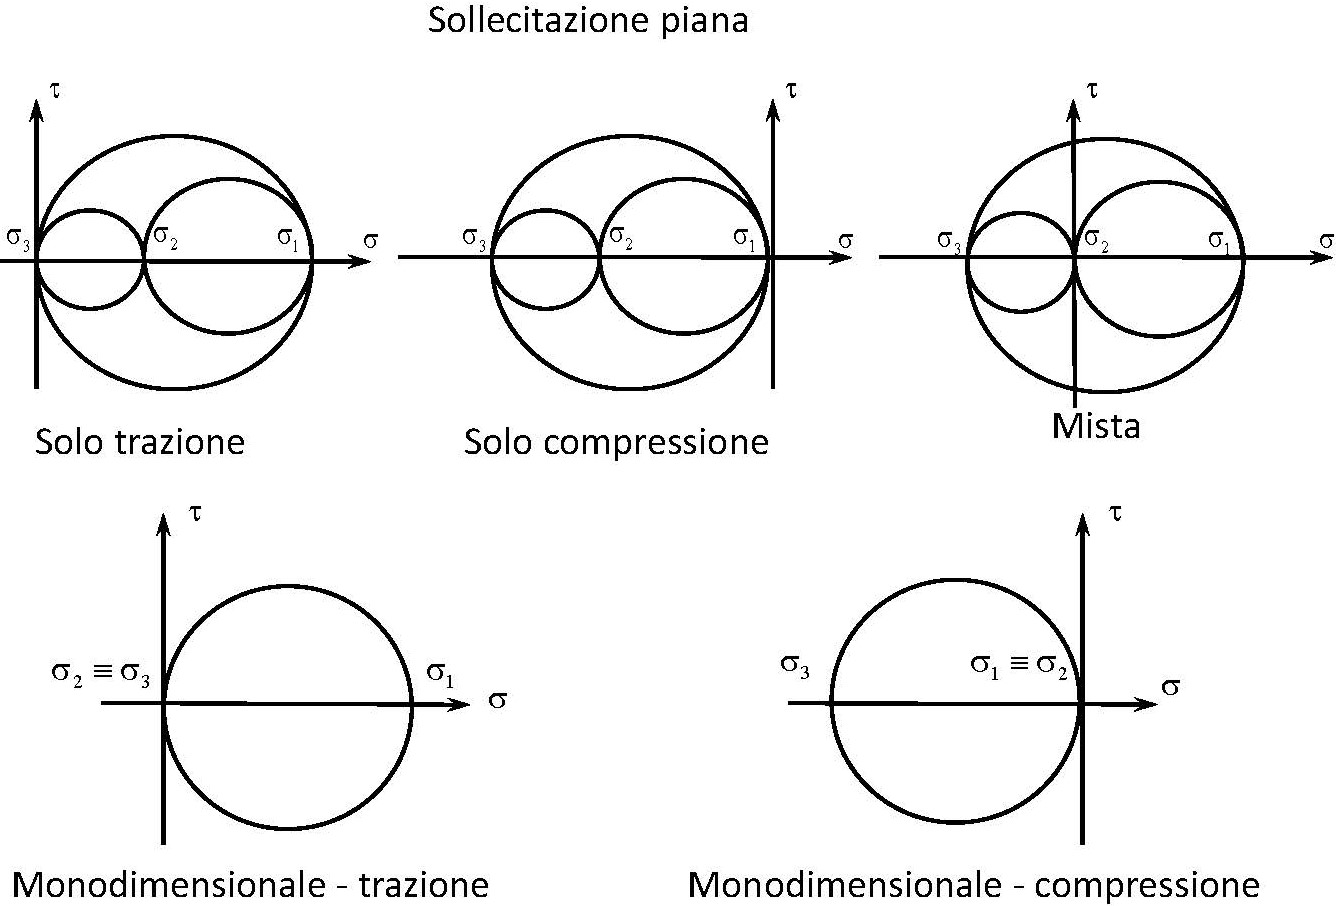
\includegraphics[width=0.8\linewidth]{immagini/1.PARTE7_Pagina_43}
\end{figure}

	\begin{oss}
		Quando si sono definite le tensioni principali era stato detto che all'interno della terna $\sigma_1,\sigma_2,\sigma_3$ ci sarà sicuramente una tensione normale che sarà la massima delle tensioni normali che si possa avere in quel punto, ovvero, se le tensioni sono ordinate come \(\sigma_1>\sigma_2>\sigma_3\) allora NON ESISTONO altre rappresentazioni del tensore delle tensioni dove $\sigma>\sigma_1$.
	\end{oss}

	Nel caso di tensione idrostatica le circonferenze degenerano in un punto. \newline

	È possibile definire i cerchi di Mohr anche per il tensore delle deformazioni di Cauchy.
	 
\newpage

{\Large \textbf{Principio del Lavori Virtuali per Corpi Deformabili}} \newline 

	Si estenda il Principio dei Lavori Virtuali definito per i corpi rigidi, a quelli deformabili, ovvero si consideri un corpo $\Omega$ soggetto a dei carichi superficiali $ p $ e di volume $ f $. \newline
	
	\begin{thm}
		Dato un corpo in equilibrio sotto l’azione di forze di volume e forze di superficie (carichi
		esterni) e delle tensioni interne, se si considera un campo di spostamenti congruente
		(che rispetta il tensore di Cauchy) il lavoro virtuale esterno deve essere uguale al lavoro
		virtuale interno.
	\end{thm}

	\begin{proof}
		Si supponga poi che il corpo, a seguito di una eventuale deformazione, raggiunga una condizione
	di equilibrio tra i carichi esterni e lo stato di tensione interno, in questo modo nel corpo si è venuta a creare una distribuzione di tensione. \newline 
	
	Gli equilibri al volume e al contorno si scriveranno: 

	\[
	\begin{aligned}
		\nabla \cdot [\sigma] + \vec{f} & = 0 \\
		\vec{p} & = [\sigma]\hat{n}
	\end{aligned}
	\]
	
	Si introduca un campo di spostamenti virtuale $ s' $ indipendenti dai carichi applicati.\newline
	
	Si introduca un campo di deformazioni che dipenda dagli spostamenti arbitrari e che sia espresso dal tensore delle deformazioni di Cauchy sotto l’ipotesi di
	garanzia della compagine. \newline
	
	Le forze applicate faranno lavoro virtuale associato agli spostamenti virtuali e dovranno essere in equilibrio.
	
	\[
	\int_{\Omega} \vec{f} \cdot \vec{s'} d\Omega + \int_{\Sigma}\vec{p} \cdot \vec{s'} d\Sigma =0
	\]
	Si vuole esprimere il seguente integrale superficiale in termini volumici:
	 \[
	 \int_{\Sigma}\vec{p} \cdot \vec{s'} d\Sigma
	 \]
	 Ricordando che il vettore $ \vec{p}$ diviene esprimibile attraverso la generica orientazione: 
	 \[
	 \begin{split}
	 	\begin{aligned}
	 	& \int_{\Sigma}\vec{p} \cdot \vec{s'} d\Sigma = \int_{\Sigma}\vec{t_n} \cdot \vec{s'} d\Sigma = \int_{\Sigma} \vec{s'} \cdot ([t] \cdot \hat{n})  d\Sigma = \int_{\Sigma}(t_{nx}u' + t_{ny} v' + t_{nz} w') d\Sigma = \\
	 	 & = \int_{\Sigma}	\left[ (t_{xx}n_x + t_{yx}n_y + t_{zx}n_z)u' + (t_{xy}n_x + t_{yy}n_y + t_{zy}n_z) v' + (t_{xz}n_x + t_{yz}n_y + t_{zz}n_z) w' \right]  d\Sigma = \\
	 	 & = \int_{\Sigma}	\left[ (\sigma_xu' + \tau_{xy}v' + \tau_{xz}w')n_x + (\tau_{yz}u' + \sigma_yv' + \tau_{zy}w')n_y + (\tau_{zx}u' + \tau_{zy}v' + \sigma_zw')n_z \right]  d\Sigma 
	 	 \end{aligned}
	 \end{split}
	 \]
	Attraverso il teorema di Gauss Green un integrale di superficie diviene un integrale di volume attraverso la sua divergenza:
	\[
	\int_{\Omega}	\left[ \dfrac{\partial}{\partial x}(\sigma_xu' + \tau_{xy}v' + \tau_{xz}w') + \dfrac{\partial}{\partial y}(\tau_{yz}u' + \sigma_yv' + \tau_{zy}w') + \dfrac{\partial}{\partial z}(\tau_{zx}u' + \tau_{zy}v' + \sigma_zw') \right]  d\Omega	
	\] 
	E dunque, infine: 
	\[
	\begin{split}	
	& \int_{\Omega} \vec{f} \cdot \vec{s'} d\Omega + \int_{\Sigma}\vec{p} \cdot \vec{s'} d\Sigma = \\
	& = \int_{\Omega} d\Omega \Biggl\{ \Bigg[u'\left( \frac{\partial \sigma_x}{\partial x} + \frac{\partial \tau_{xy}}{\partial y} + \frac{\partial \tau_{xz}}{\partial z} + f_x\right) + \\
	& + v'\left( \frac{\partial \tau_{yx}}{\partial x} + \frac{\partial \sigma_y}{\partial y} + \frac{\partial \tau_{yz}}{\partial z} + f_y\right) + w'\left( \frac{\partial \tau_{xz}}{\partial x} + \frac{\partial \tau_{yz}}{\partial y} + \frac{\partial \sigma_z}{\partial z} + f_z\right) \Bigg] +  \\
	& + \left[ \sigma_x \frac{\partial u'}{\partial x} + \sigma_y \frac{\partial v'}{\partial y} + \sigma_z \frac{\partial w'}{\partial z} + \tau_{xy} \left( \frac{\partial u'}{\partial y} + \frac{\partial v'}{\partial x}\right) + \tau_{xz} \left( \frac{\partial u'}{\partial z} + \frac{\partial w'}{\partial x}\right) + \tau_{yz} \left( \frac{\partial w'}{\partial y} + \frac{\partial v'}{\partial z}\right) \right]\Biggr\}	
	\end{split}
	\]
	
	Si noti come il termine:
	 
	 \[ \begin{split} \Bigg[ & u'\left( \frac{\partial \sigma_x}{\partial x} + \frac{\partial \tau_{xy}}{\partial y} + \frac{\partial \tau_{xz}}{\partial z} + f_x\right) + \\
	 & + v'\left( \frac{\partial \tau_{yx}}{\partial x} + \frac{\partial \sigma_y}{\partial y} + \frac{\partial \tau_{yz}}{\partial z} + f_y\right) + w'\left( \frac{\partial \tau_{xz}}{\partial x} + \frac{\partial \tau_{yz}}{\partial y} + \frac{\partial \sigma_z}{\partial z} + f_z\right) \Bigg] \end{split}\]
 
	 Rappresenti null'altro che l'equilibrio interno del corpo, sono le equazioni indefinite di equilibrio interno, essendo il corpo in equilibrio con se stesso, tale termine è nullo, perciò, il teorema del lavori virtuali si traduce in:
	 
	 \[ \begin{split}
	 \int_{\Omega} \vec{f} \cdot \vec{s'} d\Omega + \int_{\Sigma}\vec{p} \cdot \vec{s'} d\Sigma & =\int_{\Omega}  \Bigg[  \sigma_x \frac{\partial u'}{\partial x} + \sigma_y \frac{\partial v'}{\partial y} + \sigma_z \frac{\partial w'}{\partial z} + \\
	  & +\tau_{xy} \left( \frac{\partial u'}{\partial y} + \frac{\partial v'}{\partial x}\right) + \tau_{xz} \left( \frac{\partial u'}{\partial z} + \frac{\partial w'}{\partial x}\right) + \tau_{yz} \left( \frac{\partial w'}{\partial y} + \frac{\partial v'}{\partial z}\right) \Bigg] d\Omega
  		\end{split}
	 \]
	Ricordando le relazioni valide per allungamento e distorsioni si ottiene una forma finale: 
	 \[ 
		\underbrace{\int_{\Omega} \vec{f} \cdot \vec{s'} d\Omega + \int_{\Sigma}\vec{p} \cdot \vec{s'} d\Sigma}_\text{Lavoro Virtuale ESTERNO}  = \underbrace{\int_{\Omega}  \Bigg[  \sigma_x \varepsilon_x' + \sigma_y \varepsilon_y' + \sigma_z \varepsilon_z' 
		 +\tau_{xy} \gamma_{xy}' + \tau_{xz} \gamma_{xz}' + \tau_{yz} \gamma_{yz}' \Bigg] d\Omega}_\text{Lavoro Virtuale INTERNO}
	\] 
	
	\end{proof}

	Questo teorema contiene al suo interno tutto ciò che è stato fin'ora già trattato.

	\begin{itemize}
		\item Caso di corpo rigido:
		
		Campo di spostamenti: $\vec{s} = \vec{s_0} + \vec{\omega} \times \vec{r}$
		
		Tensore delle deformazioni: $[\varepsilon] = 0$
		
		\[L_V = 0\]
		
		E ci si riconduce al principio del lavori virtuali per corpi indeformabili. 
		
		\item Caso di traslazione rigida
		\[\vec{s} = \vec{s_0}\]
		\[ \left[ \int_{\Omega} \vec{f}d\Omega + \int_{\Sigma}\vec{p}d\Sigma \right] \cdot \vec{s_0} = 0 \]
		
		E si ritrovano le equazioni cardinali della statica per la traslazione.
		
		\item Caso di rotazione rigida
		
		\[  \vec{s} = \vec{\omega} \times \vec{r}\]
		
		E si ritrovano le equazioni cardinali della statica per la rotazione. 
	\end{itemize}

	\begin{oss}
		Le equazioni cardinali della statica sono contenute nel principio dei lavori virtuali:
	non è necessario imporle separatamente. \newline
	\end{oss}

	Si consideri di introdurre un incremento di spostamento $\delta s$ al corpo, ne scaturisce un incremento di deformazione $d\varepsilon, d
	\gamma$, allora avverrà anche un incremento del lavoro interno:
	
	 \[ 
	L_V = \int_{\Omega}  \Bigg[  \sigma_x \delta\varepsilon_x + \sigma_y \delta\varepsilon_y + \sigma_z \delta\varepsilon_z 
		+\tau_{xy} \delta\gamma_{xy} + \tau_{xz} \delta\gamma_{xz} + \tau_{yz} \delta\gamma_{yz} \Bigg] d\Omega
	\]
	
	Dove termine tra le parentesi rappresenta proprio l'incremento di lavoro interno specifico introdotto:
	
	\[
	L_V = \int_{\Omega} \delta \Phi d\Omega
	\]
	
	Se si considera uno spazio ideale a 6 dimensioni, ovvero le componenti di deformazione di un generico punto, allora la rappresentazione dello stato deformativo è ottenibile mediante la definizione di un punto, e muoversi da uno stato di deformazione ad un altro, in condizioni di materiale LOI, corrisponde ad uno spostamento da un punto $D_0$ ad un punto $D$ considerando un sistema di riferimento cartesiano a 6 dimensioni. \newline 
	
	In questo sistema di riferimento adottato allora può porre che durante lo spostamento da $D_0$ a $D$ si ha un incremento complessivo di lavoro interno:
	
	\[
	\Phi = \int_{D_0}^{D} \delta \Phi
	\]
	
	Tale integrale, in genere, non dipende solo da $ D_0 $ e $ D $, ma anche dal tipo di deformazione,
	ovvero dalla traiettoria tra i due punti nello spazio immaginario. \newline
	
	
	\begin{definition}
			Un corpo si dice elastico se il lavoro virtuale interno per unità di volume $ \Phi $ non dipende dal percorso di deformazione ma solo dalla configurazione iniziale e da quella finale. \newline
	\end{definition} 

	In altre parole i corpi elastici non dissipano lavoro interno (energia) lungo una trasformazione
	ciclica, durante la deformazione.
	
	\[
	 \oint \delta \Phi = 0
	\]
	
	$ \delta \Phi $ dovrà allora risultare un differenziale esatto. 
	
	Esisterà allora una funzione potenziale che
	prende il nome di \textbf{POTENZIALE ELASTICO} tale che:
	\[
	\delta \Phi = \int_{\Omega}  \Bigg[  \frac{\partial \Phi}{\partial \varepsilon_x} \delta\varepsilon_x + \frac{\partial \Phi}{\partial \varepsilon_y} \delta\varepsilon_y + \frac{\partial \Phi}{\partial \varepsilon_z} \delta\varepsilon_z 
	\frac{\partial \Phi}{\partial \gamma_{xy}} \delta\gamma_{xy} + \frac{\partial \Phi}{\partial \gamma_{xz}} \delta\gamma_{xz} + \frac{\partial \Phi}{\partial \gamma_{yz}} \delta\gamma_{yz} \Bigg] d\Omega
	\]
	Questo potenziale dovrà allora soddisfare:
	\[
	\begin{matrix}			
			\sigma_x = \dfrac{\partial \Phi}{\partial \varepsilon_x} 	& \sigma_y = \dfrac{\partial \Phi}{\partial \varepsilon_y} & \sigma_z = \dfrac{\partial \Phi}{\partial \varepsilon_z} \\
		\tau_{xy} = \dfrac{\partial \Phi}{\partial \gamma_{xy}}	& \tau_{xz} = \dfrac{\partial \Phi}{\partial \gamma_{xz}}  & \tau_{yz} = \dfrac{\partial \Phi}{\partial \gamma_{yz}} 	
	\end{matrix}
	\]
	E questa non è altro che la definizione del lavoro. \newline 
	
	Esiste quindi un legame diretto tra il campo di spostamenti e le tensioni ed è esprimibile mediante il potenziale elastico. \newline
	
	Se si definisce la quantità $\delta\Psi$ come: 
	
	\[
	\delta\Psi = \delta\sigma_x \varepsilon_x + \delta\sigma_y \varepsilon_y + \delta\sigma_z \varepsilon_z 
	+\delta\tau_{xy} \gamma_{xy} + \delta\tau_{xz} \gamma_{xz} + \delta\tau_{yz} \gamma_{yz}
	\]
	
	Allora anche  $d\Psi$ sarà un differenziale esatto: è la stessa definizione di $d\Phi$ ottenuta invertendo le grandezze. \newline
	
	La somma di due differenziali esatti sarà anch'essa un differenziale esatto: 
	\[
	\delta\Phi + \delta\Psi = \delta(\sigma_x \varepsilon_x + \sigma_y \varepsilon_y + \sigma_z \varepsilon_z 
	+\tau_{xy} \gamma_{xy} + \tau_{xz} \gamma_{xz} + \tau_{yz} \gamma_{yz}) = \delta(\Phi + \Psi)
	\]
	\[
	\Phi + \Psi = \sigma_x \varepsilon_x + \sigma_y \varepsilon_y + \sigma_z \varepsilon_z 
	+\tau_{xy} \gamma_{xy} + \tau_{xz} \gamma_{xz} + \tau_{yz} \gamma_{yz} = [\sigma]^T \cdot [\varepsilon]
	\]
	
	Chiamando ora la funzione $\Psi$ \textbf{POTENZIALE ELASTICO COMPLEMENTARE} 	
	\[
	\begin{array}{ccc}
		
		\varepsilon_x = \dfrac{\partial \Psi}{\partial \sigma_x} 	& \varepsilon_y = \dfrac{\partial \Psi}{\partial \sigma_y} & \varepsilon_z = \dfrac{\partial \Psi}{\partial \sigma_z} \\ 
		
		\gamma_{xy} = \dfrac{\partial \Psi}{\partial \tau_{xy}}	& \gamma_{xz} = \dfrac{\partial \Psi}{\partial \tau_{xz}}  & \gamma_{yz} = \dfrac{\partial \Psi}{\partial \tau_{yz}} 
		
	\end{array}
	\]
	Questo permette, mediante le derivate parziali, di ottenere il comportamento in termini di deformazione derivando il potenziale rispetto alle incognite della tensione. \newline 
	
	Il comportamento meccanico di un corpo elastico risulta quindi completamente definito se sono
	note $ \Phi $ e $ \Psi $, e allora si è in grado di ricavare il tensore delle tensioni e quello delle deformazioni. \newline
	
	Si immagini di essere in campo elastico lineare, sotto l’ipotesi di sufficiente regolarità della funzione $ \Phi $
	e quindi di continuità delle derivate seconde, il potenziale elastico nelle coordinate del tensore di Cauchy diviene:
	\[ \Phi = \Phi(\varepsilon_x, \varepsilon_y, \varepsilon_z, \gamma_{xy}, \gamma_{xz}, \gamma_{yz}) = \Phi_0 + \nabla\Phi|_0 \cdot \vec{\varepsilon} + \frac{1}{2} \vec{\varepsilon}^T H|_0 \vec{\varepsilon} + o(\varepsilon^3) \]
	
	Dove $\vec{\varepsilon}$ è il vettore delle deformazioni e i termini di $H$ sono le derivate seconde del potenziale: 
	
	\[
	h_{i,j} = \frac{\partial^2 \Phi}{\partial \varepsilon_i \partial \varepsilon_j}
	\]
	
	Se è valida l’ipotesi di piccole deformazioni l’ultimo termine diviene trascurabile. \newline
	
	Il primo termine è il potenziale elastico corrispondente allo stato indeformato, in generale
	non è nullo ma lo si considererà tale perché in questa trattazione interessano soltanto gli incrementi dello stato tensionale dovuti alle
	deformazioni; allora, sviluppando: 
	
	\[
	\nabla\Phi = \left[ \begin{array}{c}
		\dfrac{\partial \Phi}{\partial \varepsilon_x} \\
		\vdots \\
		\dfrac{\partial \Phi}{\partial \gamma_{yz}}
	\end{array}\right] = 	\left[ \begin{array}{c}
	\sigma_x \\
	\vdots \\
	\tau_{yz}
	\end{array}\right] = [\sigma] = \nabla \Phi|_0 + [H][\varepsilon]
	\]
	
	In cui il $[H][\varepsilon]$ identifica l'incremento di tensione associato alle deformazioni. \newline
	
	$ [H] $ è una matrice 6x6 reale e simmetrica che fornisce, in caso di piccole deformazioni, il legame lineare tra
	deformazioni e tensioni.
	
	\[
	[\sigma] = [H][\varepsilon]
	\]
	
	Il termine $ \nabla\Phi|_0 $ è l’aliquota costante che si ottiene per deformazione nulla e rappresenta lo stato tensionale nel materiale alla configurazione di
	partenza, rappresenta quindi la presenza di eventuali tensioni iniziali non dovute al campo di deformazioni imposto. \newline
	
	Tale termine in generale è non nullo ma lo si supporrà nullo, come analogamente fatto in
	precedenza. \newline
	
	Il potenziale si ridurrà così alla funzione quadratica:
	
	\[
	\Phi = \frac{1}{2} \vec{\varepsilon}^T H|_0 \vec{\varepsilon}
	\]

	Il comportamento elastico del corpo risulterà così completamente definito non appena saranno noti i
	21 valori numerici delle componenti della matrice $ [H] $. \newline
	
	All'interno della trattazione in cui la deformazione di un corpo è possibile solo fornendo lavoro, si impone: 
	
	\[
	\Phi([\varepsilon]) \geq 0 
	\]
	Vuol dire che se:
	\[
	\Phi = 0 \Leftrightarrow [\varepsilon] = 0
	\]
	
	Ovvero note sia le tensioni che H, si è in grado di determinare sia il potenziale elastico che le deformazioni.
	
	\[
	\begin{cases}
\begin{aligned}
[\sigma] = [H][\varepsilon] \\
\Phi = \frac{1}{2} \vec{\varepsilon}^T H|_0 \vec{\varepsilon} \geq 0
\end{aligned}
	\end{cases}
	\]
	
	Per ottenere questo prodotto necessariamente: 
	\begin{itemize}
\item $ [H] $ deve essere definita positiva;
\item I termini diagonali di $ [H] $ devono essere positivi;
\item Il determinante di $ [H] $ è non nullo (per cui il sistema è reversibile);
	\end{itemize}
	
	\[
	[\sigma] = [H][\varepsilon]
	\]
	\[
	[\varepsilon] = [H]^{-1}[\sigma]
	\]
	Sostituendo all'interno del potenziale elastico complementare si ottiene:
	\[
	\Psi = \frac{1}{2} [\sigma]^T[H]^{-1}[\sigma] = \frac{1}{2}[\varepsilon]^T[H]^{-1}[H][\varepsilon] = \frac{1}{2}[\varepsilon]^T[H]^T[\varepsilon] = \Phi
	\]
	
	Nel caso generale di elasticità valeva: 
	\[
	\Phi + \Psi = [\sigma]^T \cdot [\varepsilon]
	\]
	Aggiungendo l’ipotesi di elasticità lineare i due valori del potenziale sono
	numericamente uguali:
	\[
	\Psi = \frac{1}{2} [\sigma]^T[H]^{-1}[\sigma] = \frac{1}{2}[\varepsilon]^T[H]^T[\varepsilon] = \Phi
	\]
	\[
	\Psi = \Phi = \frac{1}{2} [\sigma]^T \cdot [\varepsilon]
	\]
	 
	Per i materiali isotropi il potenziale elastico complementare in forma generale è funzione
	delle tensioni $ xyz $:
	
	\[
	\Psi = \Psi(\sigma_x, \sigma_y, \sigma_z, \tau_{xy}, \tau_{xz}, \tau_{yz})
	\]
	
	Nel caso di materiale isotropo tutti i potenziali possono essere espressi indipendentemente dalla terna di riferimento e devono assumere lo stesso valore, e allora qualsiasi potenziale espresso in funzione delle tensioni principali avrà questa forma, in accordo col fatto che il lavoro interno deve essere indipendente dalla terna di base:
	
	\[
	\Psi = \Psi(\sigma_1, \sigma_2, \sigma_3)
	\]
	\[
	\Psi = \dfrac{1}{2} [\sigma]^T[H]^{-1}[\sigma] = \dfrac{1}{2}\left( a_{11}\sigma_1^2 + a_{22}\sigma_2^2 + a_{33}\sigma_3^2 + 2a_{12}\sigma_1\sigma_2 + 2a_{23}\sigma_2\sigma_3 + 2a_{31}\sigma_1\sigma_3\right) 
	\]

	Il potenziale deve rimanere immutato se si scambiano mutuamente le tensioni principali, per cui: 
	\[
	a_{11} = a_{22} = a_{33}
	\]
	\[
	a_{12} = a_{13} = a_{23}
	\]
	Che assumono i valori: 
	\[
	a_{ii} = \frac{1}{E} \hspace{1cm} a_{ij} = -\frac{\nu}{E}
	\]
	 In questo modo il potenziale complementare assume la seguente forma: 
	 \[
	 \Psi = \dfrac{1}{2E}\left[ \sigma_1^2 + \sigma_2^2 + \sigma_3^2 -2\nu \left( \sigma_1\sigma_2 + \sigma_2\sigma_3 + \sigma_1\sigma_3\right) \right]
	 \]
	 Accorgendosi della presenza di un quadrato di trinomio si può scrivere, per mantenere l'uguaglianza:
	\[
	\begin{split}
	\Psi & = \dfrac{1}{2E}\left[ (\sigma_x+ \sigma_y + \sigma_z)^2 -2(1+\nu) \left( \sigma_x\sigma_y + \sigma_y\sigma_z + \sigma_x\sigma_z -\tau_{xy}^2 -\tau_{xz}^2 -\tau_{yz}^2 \right) \right] = \\
	& = \dfrac{1}{2E}\left[ (\sigma_x+ \sigma_y + \sigma_z)^2 -2\nu \left( \sigma_x\sigma_y + \sigma_y\sigma_z + \sigma_x\sigma_z \right) \right] + \frac{1}{2} \frac{2(1+\nu)}{E}\left( \tau_{xy}^2 + \tau_{xz}^2 + \tau_{yz}^2\right)  
	\end{split}
	\]
	Da questa relazione si ottiene quella che lega tra loro la tensione tangenziale e il modulo di Young
	\[G = \frac{E}{2(1+ \nu)}\] 
	Allora:
	\[\frac{2(1+\nu)}{E} = \frac{1}{G}\]
	
	Derivando parzialmente il potenziale complementare si ottengono le 
	
\begin{center}
	\textbf{Equazioni Costitutive di Navier per Corpi Elastici Isotropi}
\end{center} 

Quelle che inizialmente erano state presentate come legame costitutivo. 
	\[
	\begin{cases}
		\begin{aligned}
			\varepsilon_x & = \dfrac{\partial\Psi}{\partial \sigma_x} = \dfrac{1}{E}[\sigma_x - \nu(\sigma_y + \sigma_z)] \\
			\varepsilon_y & = \dfrac{\partial\Psi}{\partial \sigma_y} = \dfrac{1}{E}[\sigma_y - \nu(\sigma_x + \sigma_z)] \\
			\varepsilon_z & = \dfrac{\partial\Psi}{\partial \sigma_z} = \dfrac{1}{E}[\sigma_z - \nu(\sigma_x + \sigma_y)] \\
			\gamma_{xy} & =  \dfrac{\partial\Psi}{\partial \tau_{xy}} = \dfrac{1}{G} \tau_{xy} \\
			\gamma_{xz} & =  \dfrac{\partial\Psi}{\partial \tau_{xz}} = \dfrac{1}{G} \tau_{xz} \\
			\gamma_{yz} & =  \dfrac{\partial\Psi}{\partial \tau_{yz}} = \dfrac{1}{G} \tau_{yz} \\
		\end{aligned}
	\end{cases}
	\]
	\[
	[\varepsilon] = [H]^{-1}[\sigma] = [C][\sigma]
	\]
	Con $ [C]$ matrice delle costanti elastiche.
	\[
	[C] = \left[ \begin{array}{cccccc}
		1/E & -\nu/E & -\nu/E & 0 & 0 & 0 \\
		-\nu/E & 1/E & -\nu/E & 0 & 0 & 0 \\
		-\nu/E & -\nu/E & 1/E & 0 & 0 & 0 \\
		0 & 0 & 0 & 1/G & 0 & 0 \\
		0 & 0 & 0 & 0 & 1/G & 0 \\
		0 & 0 & 0 & 0 & 0 & 1/G
	\end{array} \right] 
	\]
	Da questa matrice si possono fare delle osservazioni generali: 
	
	\begin{itemize}
		\item Le distorsioni sono nulle se e solo se sono nulle le tensioni tangenziali:
		\begin{itemize}
			\item Le distorsioni avvengono solo grazie alle tensioni tangenziali.
			\item Quando il materiale è lineare elastico ed isotropo lo stato di tensione e lo stato di
			deformazione presentano la stessa terna di direzioni principali. \newline 
			
			Significa dire che l'azione tangenziale e quella di distorsione sono "equivalenti", dipendono l'una dall'altra, ovvero se si ha una terna principale di tensioni in cui le $\tau$ sono nulle, di conseguenza anche le $\gamma$ saranno nulle e quella sarà una direzione principale di deformazione.
		\end{itemize}
	
		\item Le dilatazioni dipendono esclusivamente dalle tensioni normali.
		
		\item L’ipotesi di potenziale positivo si traduce in termini analitici nella condizione che la matrice
		C sia definita positiva:
		\begin{enumerate}
			\item I termini sulla diagonale devono essere positivi, ovvero devono sussistere 3 condizioni:
			\[
			\begin{cases}
				{1\over E}>0\Rightarrow E>0\\ {1\over E}>0 \Rightarrow  G>0
			\end{cases} \Rightarrow 1+\nu >0 \Rightarrow \nu >-1
			\] 
			
			\item I minori di ordine 2 devono avere determinante positivo (la più stringente delle condizioni):
			\[			
			\det\left[ \begin{array}{cc}
				1/E & -\nu/E \\
				-\nu/E & 1/E
			\end{array}\right] =  \dfrac{1}{E^2} - \dfrac{\nu^2}{E^2} = \dfrac{1}{E^2}(1-\nu^2) >0			
			\]
			\[
			(1-\nu^2) >0 \Rightarrow \nu<1
			\]
			E quindi:
			\[ -1<\nu<1\]
			\item I minori di ordine 3 devono avere determinante positivo:
			\[
			\begin{split}
				\det\left[ \begin{array}{ccc}
				1/E & -\nu/E & -\nu/E \\
				-\nu/E & 1/E & -\nu/E \\
				-\nu/E & -\nu/E & 1/E
			\end{array}\right] = \\ \dfrac{1}{E}\left[\dfrac{1}{E^2} - \dfrac{\nu^2}{E^2} \right] + \dfrac{\nu}{E}\left[-\dfrac{\nu}{E^2} - \dfrac{\nu^2}{E^2} \right]  - \dfrac{\nu}{E}\left[\dfrac{\nu^2}{E^2} + \dfrac{\nu^2}{E^2} \right]  >0
			\end{split}
			\]
			\[
			(1-\nu^2) - \nu(\nu+\nu^2) -\nu(\nu+\nu^2) >0
			\]
			\[
			(1-\nu^2) - 2\nu(\nu+\nu^2)  >0
			\]
			\[
			2\nu^3 + 3\nu^2 - 1 <0 
			\]
			Che si traduce nella condizione finale: 
			\[ -1<\nu<\dfrac{1}{2} \]
		\end{enumerate}
	\end{itemize}

\newpage 
	
{\Large \textbf{Problema dell'Equilibrio Elastico}} \mbox{} \newline

	Si è arrivati così a dimostrare il legame costitutivo di Navier. \newline 
	
	Si consideri ora il corpo $\Omega$ soggetto a carichi di volume $ f $ e superficiali $ p $ applicati sulla
	superficie $ \Sigma_p $, mentre la superficie $ \Sigma_s $ si pone essere vincolata con spostamento nullo. \newline

	Il problema risulta definito da 15 equazioni:
	\begin{itemize}
		\item 3 equazioni d'equilibrio: le equazioni indefinite di equilibrio valide su tutto il volume:
				 \[
				\begin{cases}
					\begin{aligned}
					\frac{\partial\sigma_x}{\partial x} + \frac{\partial \tau_{yx}}{\partial y} + \frac{\partial \tau_{zx}}{\partial z} + F_x & =0 \\
		
					\frac{\partial \tau_{xy}}{\partial x} + \frac{\partial\sigma_y}{\partial y} + \frac{\partial \tau_{zy}}{\partial z} + F_y & =0 \\
		
					\frac{\partial \tau_{xz}}{\partial x} + \frac{\partial \tau_{yz}}{\partial z} + \frac{\partial\sigma_z}{\partial z} + F_z & =0 \\
					\end{aligned}
				\end{cases}
				\]
				
		\item 6 equazioni costitutive del materiale del corpo: equazioni di Navier
				\[ [\varepsilon] = [C][\sigma]\]
				
		\item 6 equazioni che assicurano la congruenza del campo di spostamenti: 
				\[ 
				\begin{cases}
					\begin{aligned}
						\varepsilon_{xx} =   \frac{\partial u_x}{\partial x} \\
						\varepsilon_{yy} =   \frac{\partial u_y}{\partial y} \\
						\varepsilon_{zz} =   \frac{\partial u_z}{\partial z} \\
					\end{aligned}
				\end{cases} \hspace{1cm} \begin{cases}
					\begin{aligned}
						\gamma_{xy} =   \frac{\partial u_y}{\partial x} + \frac{\partial u_x}{\partial y} \\
						\gamma_{yz} =   \frac{\partial u_y}{\partial z} + \frac{\partial u_z}{\partial y} \\
						\gamma_{zx} =   \frac{\partial u_z}{\partial x} + \frac{\partial u_x}{\partial z} \\
					\end{aligned}
				\end{cases}
				\]
				
		\item Alle quali si aggiungono 6 equazioni al contorno: 
				\[
				3 ~ \text{su} ~ \Sigma_p \hspace{1cm} 	\begin{cases}
					p_x = \sigma_x n_x + \tau_{yx}n_y + \tau_{zx}n_z \\
					p_y = \tau_{xy}n_x + \sigma_y n_y + \tau_{zy}n_z \\
					p_z = \tau_{xz}n_x + \tau_{yz}n_y + \sigma_z n_z \\
				\end{cases}
				\]
				\[
				3 ~ \text{su} ~ \Sigma_s \hspace{1cm} u = v = w = 0
				\]
	\end{itemize}

	Le 15 equazioni correlate alle condizioni al contorno potrebbero essere sufficienti per
	determinare le 15 incognite (3 spostamenti, 6 deformazioni e 6 tensioni). \newline
	
	Ipotesi:
	\begin{itemize}
		
	 \item Materiale dal comportamento lineare elastico, isotropo, omogeneo;
	
	\item Ipotesi di piccole deformazioni e piccoli spostamenti
	\end{itemize}
	
	Il sistema può essere ridotto a 9 equazioni in 9 incognite sostituendo le equazioni di
	congruenza all’interno delle equazioni costitutive eliminando le incognite relative alle
	deformazioni:
	\[ 
	\begin{cases}
		\begin{aligned}
			\varepsilon_{xx} =   \frac{\partial u_x}{\partial x} = \dfrac{1}{E}[\sigma_x - \nu(\sigma_y + \sigma_z)] \\
			\varepsilon_{yy} =   \frac{\partial u_y}{\partial y} = \dfrac{1}{E}[\sigma_y - \nu(\sigma_x + \sigma_z)] \\
			\varepsilon_{zz} =   \frac{\partial u_z}{\partial z} = \dfrac{1}{E}[\sigma_z - \nu(\sigma_x + \sigma_y)] \\
		\end{aligned}
	\end{cases} \hspace{1cm} \begin{cases}
		\begin{aligned}
			\gamma_{xy} =   \frac{\partial u_y}{\partial x} + \frac{\partial u_x}{\partial y} = \dfrac{1}{G} \tau_{xy} \\
			\gamma_{yz} =   \frac{\partial u_y}{\partial z} + \frac{\partial u_z}{\partial y} = \dfrac{1}{G} \tau_{xz} \\
			\gamma_{zx} =   \frac{\partial u_z}{\partial x} + \frac{\partial u_x}{\partial z} = \dfrac{1}{G} \tau_{yz} \\
		\end{aligned}
	\end{cases}
	\]
	
	Alle quali si sommano le equazioni di equilibrio e le 6 equazioni al contorno. 
	\newpage
	
	Tutte le equazioni che compaiono nel sistema godono della proprietà di linearità: ci si è pur sempre posti, fin dall'inizio, in campo lineare elastico; questo vuol dire che, date $ s_1 $ e $ t_1 $ le soluzioni ai carichi applicati $ f_1 $ e $ p_1 $ e $ s_2 $ e $ t_2 $ le soluzioni associate ai carichi applicati $ f_2 $ e
	$ p_2 $, nel momento in cui si applica un sistema di carichi $ f_1+f_2 $ e $ p_1+p_2 $ si otterranno delle soluzioni che saranno rispettivamente le somme $s_1+s_2$ e $t_1+t_2$:
	
	\[
	\alpha_1f_1 + \alpha_2f_2; \alpha_1p_1 + \alpha_2p_2 \Rightarrow \alpha_1s_1 + \alpha_2s_2; \alpha_1\sigma_1 + \alpha_2\sigma_2
	\]
	
	Tale principio prende il nome di\textbf{ principio di sovrapposizione degli effetti} e vale soltanto dove le grandezze hanno tutte proprietà lineari. \newline
	
	\textit{L’effetto complessivo dovuto ad una serie di cause è uguale alla somma dei singoli effetti generati dalle cause considerate singolarmente.} \newline 

	\textbf{Principio di Kirchoff}. \textit{Al problema elastico esiste sempre una unica soluzione.} \newline 
	\begin{proof}
		Si supponga allora per assurdo che di soluzioni ne esistano due, core relativi sistemi di forze corrispondenti.
		
		\[
		f,p \rightarrow \vec{s_1},  \vec{\sigma_1}; 
		\vec{s_2}, \vec{\sigma_2} 
		\hspace{2cm} -f; -p \rightarrow -\vec{s_2}, -\vec{\sigma_2}
		\]
		\[
		f^*=0, p^*=0 \rightarrow \Delta \vec{s}, \Delta \vec{\sigma}
		\]
		Questo vuol dire che ad un sistema di forze applicato complessivo nullo corrisponde una soluzione non nulla, ovvero applicando il Principio del lavori virtuali rimane soltanto il termine:
		\[ 
		\int_{\Omega} \vec{f^*} \Delta\vec{s} d\Omega + \int_{\Sigma}\vec{p^*} \Delta\vec{s} d\Sigma = \int_{\Omega}  \Delta\vec{\sigma}^T\Delta\vec{\varepsilon} d\Omega
		\]
		Il potenziale elastico a sua volta è identicamente nullo, ma questo significa dire deformazione nulla:
		\[ 
		\int_{\Omega}  \Delta\vec{\sigma}^T\Delta\vec{\varepsilon} d\Omega = 0 = 2\int_{\Omega} \dfrac{1}{2} \Delta\vec{\sigma}^T\Delta\vec{\varepsilon} d\Omega = 2\int_{\Omega} \Phi d\Omega = 0
		\]
		Allora:
		\[
		\Phi = 0 \Rightarrow \Delta\vec{\varepsilon} = 0 \Rightarrow \Delta\vec{s} = 0\]
		La soluzione, se esiste è unica.
		\[ \vec{s_1} = \vec{s_2}	\]
	\end{proof}

	\newpage

	Si consideri un corpo inizialmente scarico a cui viene applicato un carico lentamente
	crescente fino ad una condizione di carico finale. \newline 
	
	Le forze $\vec{f}$ generano un lavoro di deformazione che sarà dato dalle forze stesse per le deformazioni che loro stesse stanno causando:
	\[
	\vec{f} = \lambda \vec{f_{fin}} \hspace{1cm} \vec{p} = \lambda \vec{p_{fin}}
	\]
	Quello che si ottiene è un vero e proprio lavoro di deformazione che ad ogni variazione di forza, in regime di linearità, risponde con un incremento di spostamento. \newline 
	
	Si definisca allora questo lavoro:
	
	\[
	L_i = \int_{\Omega}\Phi d\Omega
	\]
	\[
	L_i = \dfrac{1}{2}\int_{\Omega}\vec{\sigma}^T\vec{\varepsilon} d\Omega = \dfrac{1}{2}\left[ \int_{\Omega} \vec{f}_{fin} \cdot \vec{s} d\Omega + \int_{\Sigma}\vec{p}_{fin} \cdot \vec{s} d\Sigma 
	\right] 	\]

	In questo caso il Principio dei Lavori Virtuali è stato applicato all’integrale al primo membro e coincide con il lavoro virtuale interno compiuto dalle tensioni, ovvero gli è stato associato un sistema di deformazioni non relative alle forze esterne. \newline 
	
	\textbf{Teorema di Clapeyron}. \textit{Il lavoro di deformazione per un solido elastico lineare (il lavoro
		compiuto dalle forze di carico conseguentemente alle deformazioni provocate da loro stesse) è
		la metà del lavoro virtuale esterno (lavoro compiuto dalle stesse forze quando le stesse
		deformazioni vengono applicate ma non sono dovute alle forze stesse).}  
	
	
\newpage	

	\textbf{{\large }Esempio: trave inflessa} \newline 
	
\begin{figure}[H]
	\centering
	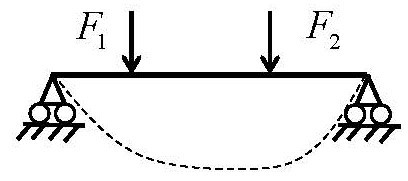
\includegraphics[width=0.3\linewidth]{immagini/1.PARTE7_Pagina_65 (3)}
	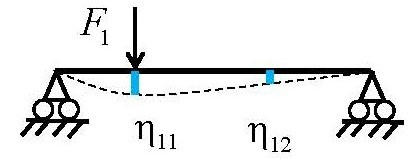
\includegraphics[width=0.3\linewidth]{immagini/1.PARTE7_Pagina_65 (4)}
	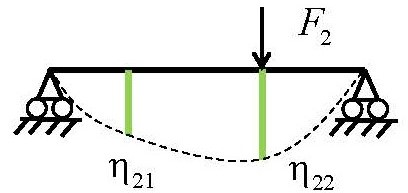
\includegraphics[width=0.3\linewidth]{immagini/1.PARTE7_Pagina_65 (5)}
	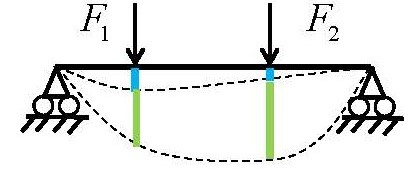
\includegraphics[width=0.3\linewidth]{immagini/1.PARTE7_Pagina_65 (6)}
\end{figure}

	Si consideri una trave appoggiata sottoposta a due carichi $ F_1 $
	ed $ F_2 $ con punti di applicazione diversi.
	Il principio di sovrapposizione è valido per tensioni e
	deformazioni, ma non è applicabile al lavoro di deformazione: tale lavoro infatti non è pari alla somma dei lavori di deformazione prodotti dalle singole forze. \newline 
	
	Sia $\eta_{ij}$ lo spostamento dovuto alla forza $ i $ nel punto di applicazione
	della forza $ j $. \newline
	
	Applicando la forza 1 e successivamente la forza 2 mantenendo
	applicata 1 si ottiene:
	\[
	L_{1,2} = \dfrac{1}{2}F_1\eta_{11} + \dfrac{1}{2}F_2\eta_{22} +F_1\eta_{21}
	\]
	Il terzo termine è null'altro che il lavoro compiuto dalla forza 1 per lo
	spostamento del punto di applicazione della stessa ma dovuto
	all’applicazione della forza 2.\newline
	
	Invertendo l'ordine di applicazione: 
	\[
	L_{2,1} = \dfrac{1}{2}F_2\eta_{22} + \dfrac{1}{2}F_1\eta_{11} +F_2\eta_{12}
	\]
	I termini $F_1\eta_{21}, F_2\eta_{12}$ sono nient'altro che lavori virtuali. \newline 
	
	Poiché in un corpo elastico il lavoro non dipende nè dal percorso
	di deformazione, nè dalla successione di carichi applicati, ne scaturisce che i due lavori devono essere uguali:
	
	\[ L_{1,2} = L_{2,1} \]
	\[ \dfrac{1}{2}F_1\eta_{11} + \dfrac{1}{2}F_2\eta_{22} +F_1\eta_{21} = \dfrac{1}{2}F_2\eta_{22} + \dfrac{1}{2}F_1\eta_{11} + F_2\eta_{12} \]
	\[ F_1\eta_{21} = F_2\eta_{12}  \]
	
	\textbf{Teorema di Betti}. \textit{Il lavoro compiuto da un sistema di forze $ F_1 $
		per gli spostamenti provocati da un secondo sistema di forze $ F_2 $
		è uguale al lavoro compiuto dal secondo sistema di forze $ F_2 $ per
		gli spostamenti provocati dal primo sistema di forze $ F_1 $} \newline 
	\newpage
{\Large \textbf{Geometria delle Aree}} \mbox{} \newline
Proprietà di una superficie delimitata da un perimetro.
\begin{figure}[H]
	\centering
	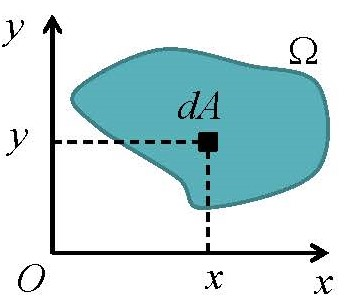
\includegraphics[width=0.25\linewidth]{immagini/1.PARTE7_Pagina_67}
\end{figure}
	Si consideri un sistema di riferimento cartesiano con $ Oxy $ ed una
	figura piana $ \Omega $. \newline

	L'area della figura sarà:
	\[
	A=\int_{\Omega} dA
	\]
	Si definisce il momento del primo ordine o \textbf{momento statico rispetto all'asse $ x $}: 
	\[
	S_x=\int_{\Omega} ydA
	\]
	Si noti come il pedice $x$ indichi l'asse rispetto al quale si misura il momento statico. \newline
	
	Si nota come l'integrale contenga la quota $y$, ovvero la distanza punto-retta del $dA$ da $x$. \newline 
	
	Analogamente si definisce il momento del primo ordine o  \textbf{momento statico rispetto all'asse $ y $}:
	\[
	S_y=\int_{\Omega} xdA
	\]
	Si definisce baricentro della figura il punto G tale che: 
	\[
	G(x_G, y_G) \hspace{1cm} \begin{cases}
								x_G = \dfrac{S_y}{A} \\
								y_G = \dfrac{S_x}{A}
	\end{cases}
	\]
	Caratteristico della figura piana, è un punto del piano che ne indica la distribuzione di area. \newline 
	
	Il baricentro della figura è invariante rispetto al sistema di riferimento: le coordinate dipendono numericamente dal sistema di riferimento ma la posizione del baricentro rimane la stessa. \newline 
	
	
\newpage
	Data una retta orientata $ r $, questa sarà individuata da un versore orientato secondo $r$ ed un versore normale. 

\begin{figure}[H]
	\centering
	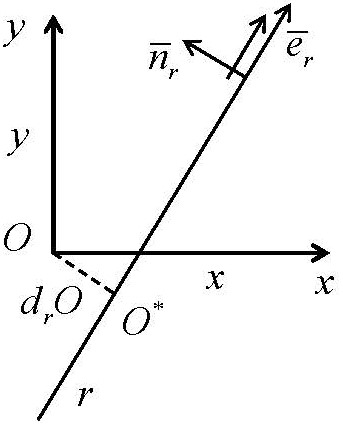
\includegraphics[width=0.25\linewidth]{immagini/1.PARTE7_Pagina_68}
\end{figure}
	Si definiscono allora:
	\begin{itemize}
		\item $ \vec{e}_r $ il versore della retta orientata $ r $
				\[ \vec{e}_r = (\alpha_x, \alpha_y, 0)\]
		\item $ \hat{n}_r $ il versore normale alla retta orientata, tale che:
				\[ \hat{n}_r = \hat{k} \times \vec{e}_r\]
				\[ \hat{k} = (0,0,1)\]
	\end{itemize}

	L’equazione che descrive i punti della retta orientata è, in forma esplicita:
	\[  -\alpha_y x + \alpha_x y + d_r O\]
	Dove $ d_r O$ è la distanza origine-retta misurata ortogonalmente alla retta stessa ed è positiva se misurata dalla stessa parte del verso positivo di $ n_r $:
	\[ d_r O>0 \Leftrightarrow (O-O^*) \cdot \hat{n_r} >0  \]
	\[ d_r O<0 \Leftrightarrow (O-O^*) \cdot \hat{n_r} <0  \]
	Allo stesso modo, qualora si volesse ricavare la distanza di un punto generico del piano dalla retta $r$, la formula è:
	\[ d_r P = -\alpha_y x_P + \alpha_x y_P + d_r O \]
	In cui i segni dei termini non possono essere modificati per non alterare l’orientamento della retta.\newline
	
	Si definisce il \textbf{Momento statico rispetto ad una retta r}:
	\[  S_r = \int_{\Omega} d_r P dA\]
	Da questa relazione si possono ricavare i momenti rispetto a $ x $ e $ y $: $ S_x $ risulterà infatti coincidente, mentre $ S_y $ di segno opposto. 
	
	Convenzionalmente si usa $ S_y $ positivo per $ x $ positive. \newline
	
	Un'altra definizione, matematica, di baricentro recita: \newline
	
	Data una distribuzione di aree $\exists! G(x_G, y_G) \Leftrightarrow \forall r : G \in r$ (retta baricentrica) $\Rightarrow  S_r = 0$ o viceversa se si ha una retta $r$ rispetto alla quale il momento statico è nullo, allora tale retta sarà baricentrica e conterrà $G$. 
	\newpage 
	Infatti se:
	\[ \begin{split}
	S_r & = \int_{\Omega} d_r P dA = \int_{\Omega} (-\alpha_y x_P + \alpha_x y_P + d_r O) dA = -\alpha_y S_y + \alpha_x S_x + Ad_r O = \\
	& = A( -\alpha_y x_G + \alpha_x y_g + d_r O) = A\cdot d_r G
	\end{split}\]
Ovvero pari alla distanza dell'asse dal baricentro della figura.

Infatti laddove $r$ fosse baricentrica, $d_r G=0$. \newline 

	L’inerzia di una figura piana rispetto ad una generica retta $ r $ è linearmente dipendente dalla
	distanza di tale retta dal baricentro $ G $ della figura. \newline
	
	Di conseguenza, sia $ G $ che $ S_r $ posso essere calcolati indipendentemente dalla terna di riferimento
	scelta.\newline

\textbf{Momenti di Inerzia (o momenti del secondo ordine)} \newline
	\begin{itemize}
			\item Momento d'inerzia rispetto all'asse x
				\[ I_x = \int_{\Omega} y^2dA \]
			\item Momento d'inerzia rispetto all'asse y
				\[ I_y = \int_{\Omega} x^2dA \]
			\item Momento centrifugo rispetto agli assi x e y
				\[ I_{xy} = \int_{\Omega} xydA \]
			\item Momento d'inerzia rispetto ad un generico asse r
				\[ I_r = \int_{\Omega} (d_r P)^2dA \]	
			\item Momento centrifugo rispetto agli assi generici r es s
				\[ I_{rs} = \int_{\Omega} (d_r P)(d_s P)dA \]		
\textbf{NB} Le distanze $Ps, Pr$ sono misurate ortogonalmente.
\begin{figure}[H]
	\centering
	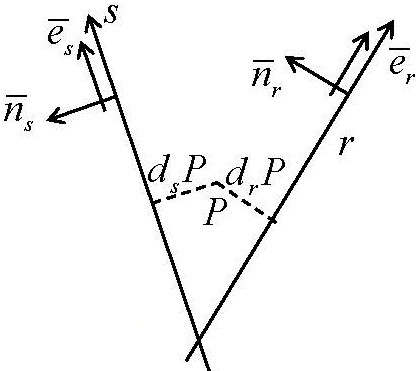
\includegraphics[width=0.25\linewidth]{immagini/1.PARTE7_Pagina_70}
\end{figure}											
	\end{itemize}
\newpage
	C'è la possibilità di scrivere gli stessi risultati ma in coordinate oblique, ovvero dati due assi coniugati, le distanze oblique vengono prese rispetto all'asse coniugato. \newline 
	
	La distanza ora non è più misurata ortogonalmente al proprio asse, ma viene presa parallelamente all'asse coniugato.  
	
	\[ I'_r = \int_{\Omega} (d'_r P)^2dA \]	
	\[ I'_{rs} = \int_{\Omega} (d'_r P)(d'_s P)dA \]
	\[  S'_r = \int_{\Omega} d'_r P dA \]
	
\begin{figure}[H]
	\centering
	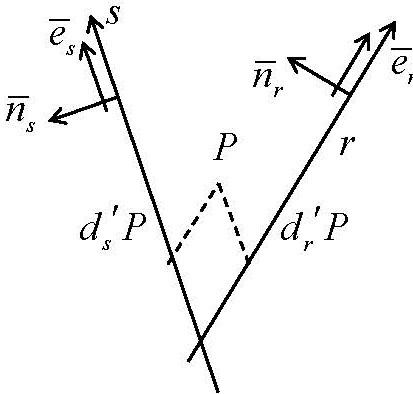
\includegraphics[width=0.25\linewidth]{immagini/1.PARTE7_Pagina_71 (2)}
	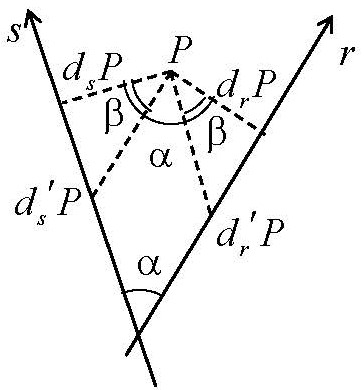
\includegraphics[width=0.25\linewidth]{immagini/1.PARTE7_Pagina_71}
\end{figure}

	\[ \beta = 90 - \alpha \hspace{1cm} \begin{cases}
										d_s P = d'_s P\cos\beta = d'_s P\sin\alpha \\
										d_r P = d'_r P\cos\beta = d'_r P\sin\alpha 
	\end{cases}\]
Per passare dalle coordinate oblique a quelle ortogonali basta moltiplicare per $\sin\alpha$. \newline

\textbf{Raggi di Inerzia} \newline
	\begin{itemize}
		\item Raggio di inerzia rispetto all’asse x
				\[ \rho_x = \sqrt{\dfrac{I_x}{A}}\]
		\item Raggio di inerzia rispetto all’asse y
				\[ \rho_y = \sqrt{\dfrac{I_y}{A}}\]	
		\item Raggio d'inerzia rispetto ad un generico asse r
				\[ \rho_r = \sqrt{\dfrac{I_r}{A}}\]	
		\item Raggio di inerzia rispetto ad un generico asse r in coordinate oblique
				\[ \rho'_r = \sqrt{\dfrac{I'_r}{A}}\]	
	\end{itemize}
\newpage
\textbf{Teorema di Huyghens-Steiner} \newline
	Qualora si volesse calcolare il momento statico rispetto ad un asse non baricentrico, basterà calcolare la distanza del baricentro dall'asse nuovo. \newline 
	
	Per quanto riguarda invece il momento d'inerzia sarà necessaria l'aggiunta di un termine di correzione.
\begin{figure}[H]
	\centering
	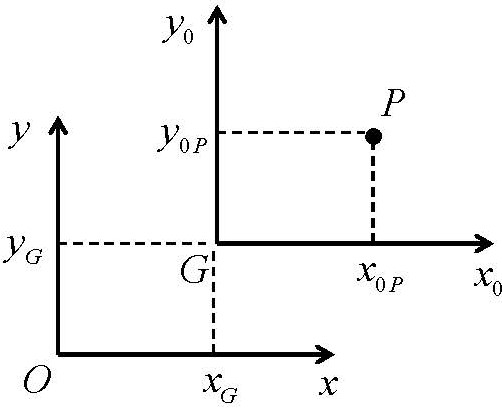
\includegraphics[width=0.25\linewidth]{immagini/1.PARTE7_Pagina_73}
\end{figure}
	\begin{thm}
		Il momento d'inerzia rispetto ad un asse $r$ generico è dato da quello rispetto $r_0$ più la distanza dal baricentro al quadrato, per l'area.
		\[  I_r = I_{r_0} + (d_rG)^2 A\]
	\end{thm}
	\begin{proof}
		Si supponga di avere due sistemi di riferimento paralleli di cui uno baricentrico.
	\[ \begin{split}
	I_x & = \int_{\Omega} y^2dA = \int_{\Omega} (y_{0P} + y_G)^2dA = \\
	    & = \int_{\Omega} y_{0P}^2dA + \int_{\Omega}y_G^2dA + \int_{\Omega}2y_G y_{0P} dA = \\
	    & = \int_{\Omega} y_{0P}^2dA + 2y_G\int_{\Omega} y_{0P} dA + y_G^2\int_{\Omega}dA  = \\
	    & = I_{x_0} + \cancel{2y_G S_{x_0}} + y_G^2A = \\
	    & = I_{x_0} + y_G^2A
	\end{split}
	\] 
	Infine: 
	\[  I_r = I_{r_0} + (d_rG)^2 A\]
	Dove $ r_0 $ è la retta parallela a $ r $ e passante per $ G $. \newline 
	
	Il teorema di Huyghens-Steiner è conosciuto anche come teorema del trasporto, ovvero, conoscendo l'inerzia rispetto ad un asse baricentrico, l'inerzia rispetto ad un asse NON baricentrico - ovvero trasportando l'asse - dev'essere corretta con un termine sicuramente positivo. \newline
	
	Il minimo momento d'inerzia si ha in corrispondenza di un asse baricentrico, qualunque altro asse darà sempre momento d'inerzia maggiore.
	\end{proof}
	
	Analogamente per il momento centrifugo:
	\[  I_xy = I_{x_0y_0} + x_Gy_G A\]
\newpage
	Si considerino ora due sistemi di riferimento baricentrici
	diversamente orientati, ruotati di $\alpha$ intorno a $z$. 

\begin{figure}[H]
	\centering
	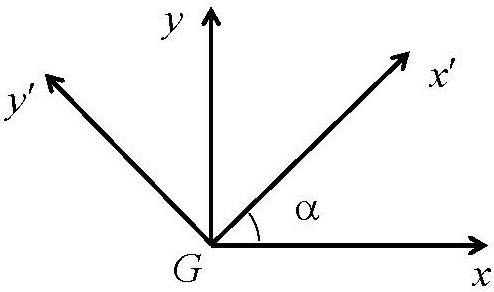
\includegraphics[width=0.25\linewidth]{immagini/1.PARTE7_Pagina_74}
\end{figure}
	La matrice di trasferimento tra i due sistemi di
	riferimento si scrive:
	\[
	T = \left[ \begin{array}{cc}
		\cos\alpha & -\sin\alpha \\
		\sin\alpha & \cos\alpha 
	\end{array}\right] 
	\]
	\[
	T^{-1} = T^T = \left[ \begin{array}{cc}
		\cos\alpha & \sin\alpha \\
		-\sin\alpha & \cos\alpha 
	\end{array}\right] \]
	Per ottenere le coordinate nel nuovo sistema di riferimento, dalla definizione, si ha:
	\[ \left[\begin{array}{c}
	x' \\
	y'
	\end{array} \right] = T^T \left[\begin{array}{c}
	x \\
	y
	\end{array} \right] = \left[ \begin{array}{cc}
	x\cos\alpha & y\sin\alpha \\
	-x\sin\alpha & y\cos\alpha 
	\end{array}\right]
	\]
	
	E i nuovi momenti d'inerzia possono quindi essere espressi come: 
	\[
	\begin{split}
		I_{x'} & = \int_{\Omega} y'^2 dA = \int_{\Omega}(-x\sin\alpha + y\cos\alpha)^2dA = \\
			   & = I_y \sin^2\alpha +I_x \cos^2\alpha - 2I_{xy}\sin\alpha\cos\alpha = \\
			   & = I_y (1-\cos^2\alpha) +I_x \cos^2\alpha - 2I_{xy}\sin\alpha\cos\alpha = I_y + (I_x - I_y)\dfrac{1+\cos2\alpha}{2}-I_{xy}\sin2\alpha = \\
			   & = \dfrac{I_x + I_y}{2} + \dfrac{I_x - I_y}{2} \cos2\alpha -I_{xy}\sin2\alpha 
	\end{split}
	\]
	Analogamente:
	\[
	\begin{split}
		I_{x'y'} & = \int_{\Omega} x'y' dA = \int_{\Omega}(x\cos\alpha + y\sin\alpha)(-x\sin\alpha + y\cos\alpha)dA = \\
		& = -I_y \sin\alpha\cos\alpha +I_x \sin\alpha\cos\alpha + I_{xy}(\cos^2\alpha - \sin^2\alpha) = \\
		& = \dfrac{I_x - I_y}{2}\sin2\alpha + I_{xy}\cos2\alpha  \\
	\end{split}
	\]
	
	Si definisce coppia di assi principali centrali di inerzia, una coppia baricentrica ortogonale che abbia il
	momento centrifugo nullo, una coppia di assi baricentrici $x,y$ rispetto alla quale $I_{xy}=0$\newline
	
	Vanno perciò cercate le soluzioni angolari all’equazione:
	\[ I_{x'y'} = \dfrac{I_x - I_y}{2}\sin2\alpha + I_{xy}\cos2\alpha = 0 \]
	Al variare di $\alpha$ esisterà una coppia $x'y'$ tali che $I_{xy}=0$ \newline
	
	\begin{itemize}
		\item Si possono avere infinite coppie di assi principali se il momento centrifugo è già nullo:
	\[ I_{xy} = 0 \hspace{1cm} I_x = I_y \Rightarrow \forall \alpha\]
	È una condizione sempre verificata, c'è sempre una terna principale d'inerzia, tutte le terne ottenute per rotazione intorno all'asse $z$ rispetto al sistema di riferimento $x,y,z$ sono terne principali: tutte le coppie $x,y$ sono coppie di assi principali. 
	
	\item Si ottiene un Unico riferimento principale centrale se:
	\begin{itemize}
	\item	\[ I_{xy} = 0 \hspace{1cm} I_x \ne I_y \Rightarrow  \alpha = k\dfrac{\pi}{2}\]
	Per trovare le altre coppie principali basterà ruotare di $\alpha$ il sistema di riferimento 
	
	\item\[ I_{xy} \ne 0 \hspace{1cm} I_x = I_y \Rightarrow  \alpha = \dfrac{\pi}{4} + k\dfrac{\pi}{2}\]
	
	\item \[ 
	I_{xy} \ne 0 \hspace{1cm} I_x \ne I_y \Rightarrow  \alpha = \dfrac{1}{2}\arctan\dfrac{2I_{xy}}{I_y - I_x} + k\dfrac{\pi}{2} 
	\]
	Questo è il caso più generale possibile, vuol dire che sostanzialmente  a partire da una coppia di assi $x,y$, con la relazione trovata per $\alpha$ si è in grado di ricostruire la rotazione necessaria per ottenere un sistema di riferimento principale. 
	\end{itemize}
	\end{itemize}

	Si ricavino ora queste proprietà delle aree per particolari forme comuni. \newline

{\Large \textbf{Rettangolo}} \mbox{} \newline
\begin{figure}[H]
	\centering
	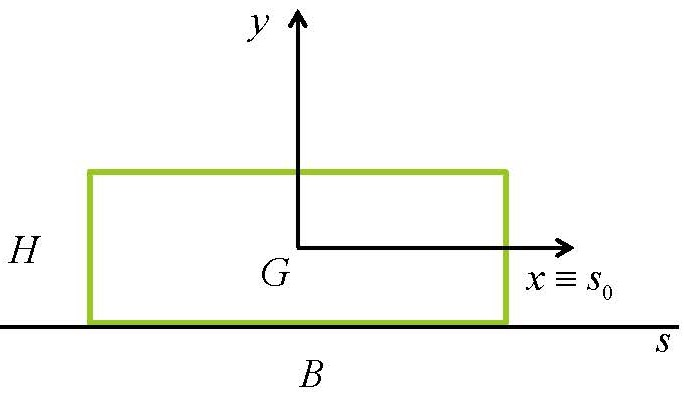
\includegraphics[width=0.25\linewidth]{immagini/1.PARTE7_Pagina_76}
\end{figure}

	Il baricentro G è un'indicazione della distribuzione di superficie, qualora esistano degli assi di simmetria, $G$ si troverà su tali assi, se ne esistono due $G$ è univocamente definito come l'intersezione di tali assi. \newline 
	
	Il momento di prim'ordine 
	\[ S_r = \int_{\Omega} (d_rP)dA\]
	È nullo se r è di simmetria, d'altro canto il dominio è simmetrico. 
	\[S_s = A (d_sG) = BH\dfrac{H}{2} = \dfrac{BH^2}{2}\]
	Inoltre se r è di simmetria ortogonale, r e la sua
	perpendicolare sono coniugati e baricentrici,
	quindi sono assi principali di inerzia. \newline
	
	Va al cubo la componente rispetto alla quale si sta calcolando il momento $I$. 
	
	\[I_x \Rightarrow y \hspace{1cm} I_y \Rightarrow x\]
	
	\[ I_{s_0} = \int_{-B/2}^{B/2} \int_{-H/2}^{H/2} y^2 dxdx = \dfrac{BH^3}{12}\]
	
	\[ I_s = I_{s_0} + A(d_sG)^2 = \dfrac{BH^3}{12} + BH \left( \dfrac{H}{2} \right)^2 = \dfrac{BH^3}{3} \]
	
	\[ \rho_x = \sqrt{\dfrac{I_x}{A}} = \sqrt{\dfrac{I_{s_0}}{A}} = \dfrac{H}{\sqrt{12}} \hspace{1cm} \rho_y = \sqrt{\dfrac{I_y}{A}} = \dfrac{B}{\sqrt{12}} \hspace{1cm} I_{xy} = \int_{\Omega}xydA = 0 \]
	
	Questa è una terna principale d'inerzia, qualora si abbia un asse di simmetria e quindi baricentrico, tale asse non è soltanto baricentrico ma anche principale d'inerzia. 
	
	L'asse di simmetria è asse principale d'inerzia e il suo coniugato sarà anch'esso principale d'inerzia.  \newline
	
{\Large \textbf{Cerchio}} \mbox{} \newline
\begin{figure}[H]
	\centering
	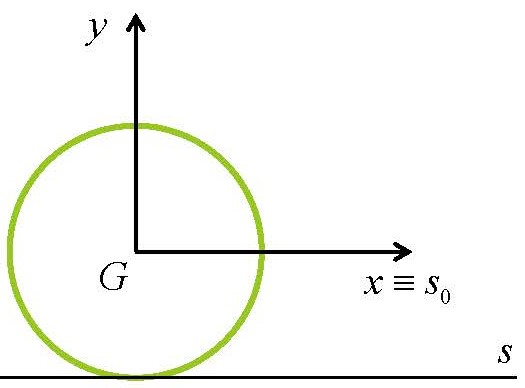
\includegraphics[width=0.25\linewidth]{immagini/1.PARTE7_Pagina_77}
\end{figure}
	Il baricentro G è un'indicazione della distribuzione di superficie, qualora esistano degli assi di simmetria, $G$ si troverà su tali assi, se ne esistono due $G$ è univocamente definito come l'intersezione di tali assi. \newline 
	
	Si definisce inerzia polare, l'inerzia rispetto all'asse ortogonale al piano su cui giace la figura. 
	\[I_p = I_x + I_y\] 
	Se non c'è differenza di distribuzione d'area $ I_x = I_y $ e allora si può scrivere:
	\[ I_p = 2I_x\]
	
	Il momento del prim'ordine:
	\[ S_r = \int_{\Omega} (d_rP)dA\]
	È nullo se r è di simmetria, d'altro canto il dominio è simmetrico. 
	\[S_s = A (d_sG) = \pi R^2R = \pi R^3\]
	Inoltre se r è di simmetria ortogonale, r e la sua
	perpendicolare sono coniugati e baricentrici,
	quindi sono assi principali di inerzia. \newline 
	
	\[ I_{s_0} = \int_{-R}^{R} \int_{-R}^{R} y^2 dxdx = \dfrac{I_p}{2}=\dfrac{\int_{0}^{R}r^2dA}{2} \overset{dA=rd\theta}{=} \dfrac{\int_{0}^{R}2\pi r^3dr}{2} = \dfrac{\pi R^4}{4} = \dfrac{\pi D^4}{64}\]
	
	\[ I_s = I_{s_0} + A(d_sG)^2 = \dfrac{\pi R^4}{4} + \pi R^4 = \dfrac{5\pi R^4}{4} \]
	
	\[ \rho_x = \sqrt{\dfrac{I_x}{A}} = \dfrac{R}{2} \hspace{1cm} \rho_y = \sqrt{\dfrac{I_y}{A}} = \dfrac{R}{2} \hspace{1cm} I_{xy} = \int_{\Omega}xydA = 0 \]
	Per un cerchio qualunque asse baricentrico è asse principale d'inerzia. \newline
	
	Gli assi x e y sono principali di inerzia.
	
\newpage
	Per quanto riguarda la geometria delle aree si possono sfruttare le operazioni Booleane, ovvero si può operare con le aree per somma e sottrazione e riversare queste operazioni sulle grandezze relative ai momenti d'inerzia. \newline
	
{\Large \textbf{Settore Circolare}} \mbox{} \newline
	Per cui l'inerzia di 1/4 di cerchio sarà 1/4 del momento d'inerzia del cerchio rispetto allo stesso asse $s$ passante per il baricentro della figura. 

	Quella che però cambia è la distribuzione di area, il baricentro della figura tagliata non è più coincidente con quello della figura intera, per cui, per trovare il vero momento d'inerzia, si sfrutterà il teorema di Huyghens-Steiner al contrario,:si sta ricercando l'inerzia rispetto all'asse baricentrico. 
\begin{figure}[H]
	\centering
	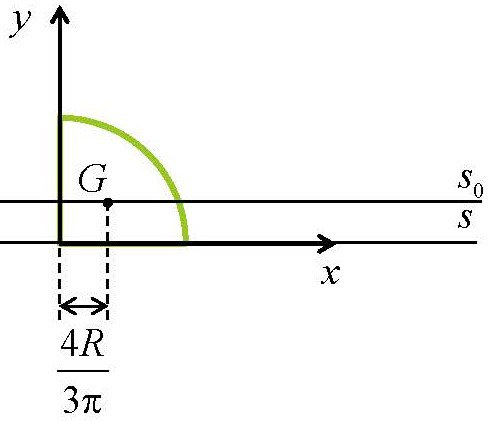
\includegraphics[width=0.25\linewidth]{immagini/1.PARTE7_Pagina_78 (2)}
\end{figure}
	
	Come detto momento di inerzia di un settore circolare è un quarto di quello del cerchio di partenza rispetto all’asse passante per il
	baricentro del cerchio stesso.
	
	\[ I_{s} = \dfrac{1}{2}\dfrac{\pi R^4}{4} = \dfrac{\pi R^4}{16}\]
	
	\[ I_{s_0} = I_{s} - A(d_sG)^2 = \dfrac{\pi R^4}{16} - \dfrac{\pi R^2}{4} \left( \dfrac{4R}{3\pi}\right)^2 = \dfrac{\pi R^4}{16}  - \dfrac{4R^4}{9\pi} \]
	
{\Large \textbf{Triangolo Rettangolo}} \mbox{} \newline
	Un triangolo rettangolo è la metà di rettangolo ottenuto tagliando il rettangolo lungo una sua diagonale. \newline 
	
	Il suo momento d'inerzia sarà perciò la metà.
\begin{figure}[H]
	\centering
	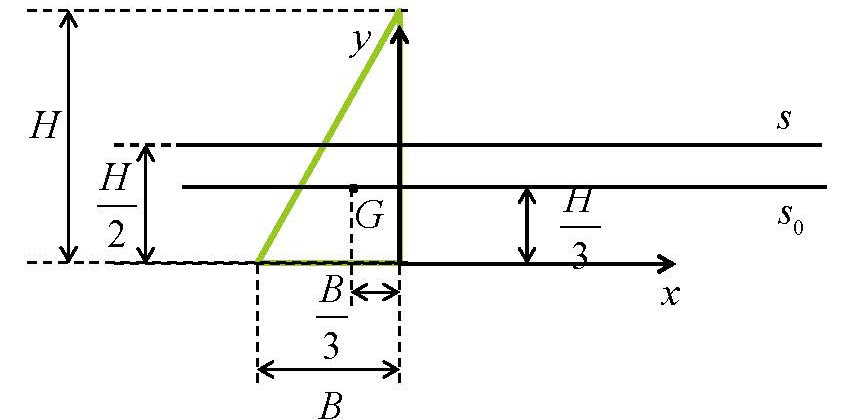
\includegraphics[width=0.25\linewidth]{immagini/1.PARTE7_Pagina_78}
\end{figure}
	Analogamente a quanto fatto con settore circolare.
	
	\[ I_{s} = \dfrac{BH^3}{24}\]
	
	\[ I_{s_0} = I_{s} - A(d_sG)^2 = \dfrac{BH^3}{24} - \dfrac{BH}{2} \left( \dfrac{H}{6} \right)^2 = \dfrac{BH^4}{36} \]
	\newpage
{\Large \textbf{NOTE}} \mbox{} \newline	


%\vfill
%\begin{tcolorbox}[height=4.5cm]
%	This box has a height of 1cm.
%\end{tcolorbox}

\end{adjustwidth}
\end{document}